\documentclass[conference,compsoc]{IEEEtran}
% \IEEEoverridecommandlockouts

\renewcommand\thesection{\arabic{section}}
\renewcommand\thesubsection{\thesection.\arabic{subsection}}
\renewcommand\thesubsubsection{\thesubsection.\arabic{subsubsection}}

\renewcommand\thesectiondis{\arabic{section}}
\renewcommand\thesubsectiondis{\thesectiondis.\arabic{subsection}}
\renewcommand\thesubsubsectiondis{\thesubsectiondis.\arabic{subsubsection}}

% The preceding line is only needed to identify funding in the first footnote. If that is unneeded, please comment it out.
\usepackage{cite}
\usepackage{amsmath,amssymb,amsthm,amsfonts}
\usepackage{algorithmic}
\usepackage{graphicx}
\usepackage{textcomp}
\usepackage{xcolor}
\usepackage{listings}
\usepackage[ruled]{algorithm2e}
\usepackage[explicit]{titlesec}
\def\BibTeX{{\rm B\kern-.05em{\sc i\kern-.025em b}\kern-.08em
    T\kern-.1667em\lower.7ex\hbox{E}\kern-.125emX}}

% Our custom theorems/properties
\newtheorem{prp}{Property}
% \newtheorem{proofprp}{}

% TODO
\newtheorem{subprp}{Property}[prp]
\newtheorem{thm}[subprp]{Theorem}
\newtheorem{defn}[subprp]{Definition}

% -----------------------------------------------------------------
%                   end header
%------------------------------------------------------------------

\begin{document}
\title{An Improved K-Means Clustering Algorithm for One Dimensional Data}

\author{\IEEEauthorblockN{Ryan Froese}
\IEEEauthorblockA{\textit{Dept. of Computer Science} \\
\textit{University of Manitoba} \\
Winnipeg, MB, Canada \\
froeser5@myumanitoba.ca}
\and

\IEEEauthorblockN{James Klassen}
\IEEEauthorblockA{\textit{Dept. of Computer Science} \\
\textit{University of Manitoba} \\
Winnipeg, MB, Canada \\
klass167@myumanitoba.ca}
\and

\IEEEauthorblockN{Tyler Loewen}
\IEEEauthorblockA{\textit{Dept. of Computer Science} \\
\textit{University of Manitoba} \\
Winnipeg, MB, Canada \\
loewent4@myumanitoba.ca}
}

\maketitle

\begin{abstract}
Clustering is a widely used technique for data pre-processing, mining, and analysis. The k-means clustering algorithm is commonly used because of its simplicity and flexibility to work in many data mining domains. Despite being commonly used, the k-means algorithm suffers from non-deterministic results and run times that vary greatly depending on the initial selection of cluster centroids. There have been many proposed improvements to the k-means algorithm. We propose the f-cluster algorithm which combines concepts from the k-means algorithm with an additional focus on the concepts of the borders dividing clusters. What we find is deterministic results with greatly improved run time over the k-means algorithm.
\end{abstract}

\begin{IEEEkeywords}
Clustering algorithms, Cluster analysis, k-means algorithm, Data analysis
\end{IEEEkeywords}

\section{Introduction}

Clustering is a data mining technique used to arrange large amounts of data into distinct clusters. It is used in many fields including image processing, pattern recognition, bioinformatics, spatial data analysis, and more. The idea of a clustering algorithm is to create clusters containing data points from a dataset where every data point in the same cluster is more similar to one another than to the data points in other clusters (i.e., maximizing the intra-class similarities within a cluster and minimizing inter-class similarities between other clusters). Thus, creating a set of data points in a cluster that are locally more similar to each other than to data points in other clusters. Clustering can help researchers better understand the distribution and structure of large datasets. In Section 2 we introduce the partitioning approach to clustering and describe the k-means clustering algorithm along with some of its shortcomings. We then discuss some commonly used approaches to improving the k-means algorithm. In Section 3 we propose our improved k-means algorithm. We include pseudo code for our algorithm, a formal proof of correctness, and the time complexity of a single iteration. In Section 4 we analyze the experimental results of our algorithm and compare both artificial datasets of different sizes and distributions, and a real-world dataset. In Section 5 we use a real-world dataset containing oceanic and atmospheric data combined with our clustering algorithm to visualize geospatial data. We also discuss any new findings and relationships that become apparent when visualizing the data. Lastly, Section 6 provides a summary of our findings, visualizations of our dataset and potential improvements to our algorithm in the future.

\section{Background}

\subsection{Clustering}

There are three major techniques for clustering: partitioning methods, hierarchical methods, and density-based methods. The partitioning method is used by the original k-means algorithm and our algorithm. The partitioning method takes a dataset of size $n$ and partitions it into some $k$ number of partitions (clusters) where $k \leq n$. Each cluster contains at least one data point, and each data point belongs to exactly one cluster (i.e., distinct clusters). The similarities between items in each cluster are then evaluated using a distance function through an iterative process until all data points are in their current cluster. The centre of a cluster can be calculated using the centroid or medoid methods. The centroid of a cluster is determined by calculating the average of every data point in the cluster while the medoid of a cluster is determined by calculating the median data point of the cluster.

\subsection{k-means Clustering Algorithm}

The k-means algorithm is a widely used clustering algorithm that is easy to understand and implement and can be used across a large variety of problems \cite{b1, b2, b3, b4, b5}. We have included the pseudo code of the k-means algorithm as Algorithm 1 for reference. There are two phases in the k-means algorithm. During the initial phase, $k$ random values are chosen from the dataset and assigned as the initial centroids of each of the clusters where $k$ is the number of clusters \cite{b1}. In the second phase, the distance from each data point in a cluster to the centroid of every other cluster is calculated. If a data point is closer to a different cluster than the one it currently belongs to, the data point is moved to the closest cluster. After one iteration is complete and all data points have been moved, the centroids for each cluster are recomputed. This process continues until none of the data points move to a different cluster which occurs when the centroids of each cluster do not change. One of the issues with the k-means algorithm is the random selection of initial cluster centroids. This random selection has two main effects on the behaviour of the algorithm. First, it makes the algorithm non-deterministic in the final clusters it produces \cite{b1}. This means the number of data points in each cluster can vary greatly depending on the initial centroids chosen. Second, for large datasets, some random selections of initial centroids can greatly reduce the performance of the algorithm as more iterations are required to move data points between clusters \cite{b1, b2}.

\begin{algorithm}\label{alg-1}
    \caption{k-means clustering algorithm}
    Input:
        \begin{itemize}
            \item $D = \{d_1, d_2, \dots, d_n\}$: Set of $n$ data points in any order
            \item $k$: Number of clusters
        \end{itemize}
    Output:
        \begin{itemize}
            \item A set of $k$ clusters
        \end{itemize}
    Steps:
        \begin{enumerate}
            \item Randomly select $k$ data points from $D$ as initial centroids
        \end{enumerate}
        Repeat until values of centroids do not change:
        \begin{enumerate}
        \setcounter{enumi}{1}
            \item Assign each data point $d_i$ to the cluster with the closest centroid
            \item Calculate the new centroid of each cluster
        \end{enumerate}
\end{algorithm}

\subsection{Related Work}

There have been many improvements to the k-means clustering algorithm \cite{b1, b2, b3}. The global k-means clustering algorithm modifies the k-means algorithm by minimizing the distance between data points within the same cluster using the k-means algorithm as a local search procedure \cite{b2}. In this algorithm, the local k-means algorithm starts with a single cluster and calculates the centroid of this cluster. The global k-means algorithm then applies the k-means algorithm sequentially on an increasingly large number of clusters to solve a local problem \cite{b2}. At the start of each local search, the cluster centroids are initially placed at the currently most optimal position, which is determined by the centroids calculated in the previous iteration’s local search \cite{b2}. This improves performance by reducing the number of data points that have to be moved between clusters. The global k-means algorithm produces deterministic results because it starts with a single cluster and computed centroid. It also has improved performance over the k-means algorithm because it always passes the most recently calculated centroid(s) of the current iteration to the next iteration, reducing the number of data points that are moved between clusters \cite{b2}.

The improved k-means algorithm proposed by K. Nazeer and M. P. Sebastian \cite{b1} modifies the original k-means algorithm using a technique to systematically determine the initial centroids of each cluster with better accuracy than when selecting them randomly \cite{b1}. The clustering process is then applied to the initial clusters using a heuristic approach for improved efficiency \cite{b1}. In this heuristic approach, the distances from each data point in a cluster to their nearest cluster are saved and passed to the next iteration. In the next iteration the distances from the previous iteration are compared to the new distances from each data point in the cluster to the cluster they are closest to. If the distance calculated in the current iteration is less than or equal to the distance calculated in the previous iteration then the data point stays in its current cluster. Otherwise, the distance from the data point to every other cluster is calculated to find the new closest cluster to the data point.

\section{Modified Approach}

\subsection{f-Clustering algorithm}

In this paper, we propose the f-cluster algorithm, a modified version of the original k-means algorithm optimized for single-dimensional data. The f-cluster algorithm has two phases. In the first phase, we use Algorithm 2 to determine the initial cluster centroids which are used in Algorithm 3. To get the initial cluster centroids, Algorithm 2 sorts the data points in ascending order in Step 1 and assigns a centroid value to each $k$ clusters by choosing $k$ data points evenly distributed across the dataset in Step 2. In Step 3, we iterate over each data point exactly once and assign it to the cluster it is closest to. The initial centroids are recalculated in Step 4 to account for data points that have changed clusters in Step 3. Lastly, Step 5 returns the list of initial centroids, a list of the sum of data point values in each cluster, and the number of data points in each cluster.

\begin{algorithm}\label{alg-2}
    \caption{Finding initial centroids}
    Input:
        \begin{itemize}
            \item $D = \{d_1, d_2, \dots, d_n\}$: Set of $n$ data points in any order
            \item $k$: Number of clusters
        \end{itemize}
    Output:
        \begin{itemize}
            \item $C = \{c_1, c_2, \dots, c_k\}$: Set of initial cluster centroids in ascending order
            \item $S = \{s_1, s_2, \dots, s_k\}$: The sum of data point values in each cluster
            \item $N = \{n_1, n_2, \dots, n_k\}$: The number of data points in each cluster
        \end{itemize}
    Steps:
        \begin{enumerate}
            \item Sort $D$ in ascending order
            \item Define $C$ as a linear interpolation with $k$ data points beginning with $d_1$ and ending with $d_k$
            \item For each data point $d_i$:
            \begin{itemize}
                \item Determine the cluster centroid closest to $d_i$
                \item Add the value of $d_i$ to the appropriate element in $S$
                \item Increment the count of the appropriate element in $N$
            \end{itemize}
            \item Re-calculate each centroid $c_i \in C$ as $\frac{s_i}{n_i}$
        \end{enumerate}
\end{algorithm}


In the second phase, we use Algorithm 3 which takes the output of Algorithm 2 and determines the final clusters. Step 1 calculates the positions of the cluster borders by using the number of data points in each cluster as seen in Eq.(1). Once the cluster borders are calculated we calculate the initial average of the cluster border in Step 2 using the centroids of the two clusters neighbouring the cluster border. Step 3 is an iterative looping process that moves the cluster borders one position at a time until they are in the correct position. Step 3 is executed on each cluster border sequentially, only moving the next cluster border when the current cluster border is in the correct position. There are three cases to consider in Step 3. In case 3a, the cluster border continues to move one position to the left as long as the data point to the left of the cluster border is greater or equal to the cluster border average. In case 3b the cluster border continues to move one position to the right as long as the data point to the right of the cluster border is less than the cluster border average. In both case 3a and case 3b, the cluster border will no longer be moved when case 3c is true. In case 3c the cluster border is in the correct position because the data point directly to the left of the cluster border is less than the cluster border average and the data point immediately to the right of the cluster border is greater or equal to the cluster border average. When this is the case, the algorithm continues to the next cluster border. When case 3c is true for every cluster border, then all data points are in the correct clusters; this is the terminating condition of Algorithm 3. When Step 3 has terminated, any clusters containing no data points are removed in Step 4. Then in Step 5, the centroid of each cluster is updated using the cluster sums and cluster counts lists. Since each cluster sum and count is updating continuously in Step 3, calculating the centroids in Step 5 is trivial and does not require iterating over every data point. Finally, Step 6 outputs the list of centroids, sums of each cluster, and the number of items in each cluster.


\begin{algorithm}\label{alg-3}
    \caption{f-cluster algorithm}
    Input:
        \begin{itemize}
            \item $D = \{d_1, d_1, \dots, d_n\}$: Set of $n$ data points in ascending order
            \item $k$: Number of clusters
            \item $C = \{c_1, c_2, \dots, c_k\}$: Initial set of cluster centroids in ascending order
            \item $S = \{s_1, s_2, \dots, s_k\}$: The sum of data points values in each cluster
            \item $N = \{n_1, n_2, \dots, n_k\}$: The number of data points in each cluster
        \end{itemize}
    Output:
        \begin{itemize}
            \item $C = \{c_1, c_2, \dots, c_k\}$: Updated centroids for each cluster
            \item $S = \{s_1, s_2, \dots, s_k\}$: Updated sums of data points values in each cluster
            \item $N = \{n_1, n_2, \dots, n_k\}$: Updated numbers of data points in each cluster
        \end{itemize}
    Steps:
        \begin{enumerate}
            \item Determine the indexes that divide each cluster using $N$.
            \item Compute the cluster border averages by taking the average of the cluster centroids adjacent to each cluster border.
            \item Repeat for each cluster border $b_i$:
            \begin{enumerate}
                \item If the data point immediately before $b_i$ is greater than or equal to the corresponding adjacent cluster border average, move $b_i$ to the left until this is no longer the case. Update the appropriate elements in $S$ and $C$ for each cluster.
                \item If the data point immediately after $b_i$ is less than the corresponding adjacent cluster border average, move $b_i$ to the right until this is no longer the case. Update the appropriate elements in $S$ and $C$ for each cluster.
                \item If the data point immediately before $b_i$ is less than the corresponding adjacent cluster border average, and the data point immediately after the cluster border is greater than or equal to the corresponding adjacent cluster border average, $b_i$ is in the correct position.
            \end{enumerate}
            \item Delete any empty clusters.
            \item Update each $c_i \in C$ as $\frac{s_i}{n_i}$.
        \end{enumerate}
\end{algorithm}


Algorithm 4 is the complete algorithm that combines Algorithm 2 and Algorithm 3. As input, Algorithm 4 takes an unsorted dataset and some number of clusters $k$ and outputs a list of cluster centroids. In phase 1, we use Algorithm 2 to determine the initial cluster centroids as well as the sum and number of data points in each cluster. These outputs are then used in phase 2 where Algorithm 3 performs the full clustering which produces a list of cluster centroids.

% -----------------------------------
% START HERE
% -----------------------------------

\begin{algorithm}\label{alg-4}
    \caption{Full clustering algorithm}
    Input:
        \begin{itemize}
            \item $D = \{d_1, d_1, \dots, d_n\}$: Set of $n$ data points in any order
            \item $k$: Number of clusters
            \item $C = \{c_1, c_2, \dots, c_k\}$: List of cluster centroids
        \end{itemize}
    Output:
        \begin{itemize}
            \item $C = \{c_1, c_2, \dots, c_k\}$: List of cluster centroids
        \end{itemize}
    Steps:
        \begin{enumerate}
            \item Use Algorithm 2 to determine the initial cluster centroids, cluster sums, and cluster data point counts
            \item Use output from Algorithm 2 as input to Algorithm 3 to determine $C$ 
        \end{enumerate}
\end{algorithm}


\subsection{Proof of Correctness}

In this section we prove the following two properties of the f-cluster algorithm to show that the algorithm always produces the correct results:
\begin{prp}\label{closest-centroid}Each data point in the dataset will be assigned to the cluster it is closest to\end{prp}
\begin{prp}\label{border-cross}The cluster borders cannot cross each other as this would cause the sum and count calculations to be incorrect.\end{prp}

For the algorithm to work correctly we assume that there are no duplicate centroids. When a data point has an equal distance to two different centroids we assign the data point to the cluster with the larger of the two centroids. This behaviour is omitted from the proof because the probability of two distances being equal considering floating-point precision is very low. We also assume that there are at least two clusters, that is $k \geq 2$. For future reference in this proof, cluster borders are positions that separate the data points into clusters by defining where clusters begin and end in the dataset.

\subsubsection{Setup}
Algorithm inputs:
\begin{itemize}
\item $D = \{d_{11}, d_{12}, \dots , d_{1n_1}, \dots, d_{kn_k}\}$: Dataset with elements $d_{ij}$ where $i$ is the cluster and $j$ is the index within the cluster
\item $k$: Number of clusters where $k \geq 2$
\item $C = \{c_1, \dots, c_k\}$: Set containing the centroids of each cluster where each $c$ is unique and $c_1 < c_2 < \dots < c_k$
\item $S = \{s_1, \dots, s_k\}$: Set containing the sums of data points in each cluster
\item $N = \{n_1, \dots, n_k\}$: Set containing the number of data points in each cluster
% \item $N_{\text{sum}} = {n_1 + \dots + n_k}$ where $N_{\text{sum}}$ is the total number of data points in $D$
\end{itemize}

To better visualize the intuition of the algorithm, we model the data and associated clusters as a sorted list of data points in clusters separated by cluster borders, i.e. the first border separates clusters 1 and 2, etc.. The set of all cluster borders positions is defined as$B = \{b_1, \dots, b_{k-1}\}$. The algorithm inputs and borders can be visually represented by Eq.(1).

\begin{equation}\label{alg-vis}\begin{aligned}
D=
\underbrace{d_{11}, d_{12}, \dots, d_{1x_1}}_{\substack{s_1 = d_{11} + \dots + d_{1x_1} \\  c_1 = \frac{s_1}{x_1}}}
\overbrace{|}^{\substack{b_1 = \\ x_1}}
% \\
\underbrace{d_{21}, d_{22}, \dots, d_{2x_2}}_{\substack{s_2 = d_{21} + \dots + d_{2x_2} \\  c_2 = \frac{s_2}{x_2}}}
\overbrace{|}^{\substack{b_2 = \\ x_1 + x_2}}
\dots \\
\overbrace{|}^{\substack{b_{k-1} = \\ x_1 + x_2 + \dots + x_{k-1}}}
\underbrace{d_{k1}, d_{k2}, \dots, d_{kx_k}}_{\substack{s_k = d_{k1} + \dots + d_{kx_k} \\  c_k = \frac{s_k}{x_k}}}
\end{aligned}
\end{equation}

\subsubsection{Outline of Proof of Property \ref{closest-centroid}}

\textbf{Property 1.1}: Data points can only be closest to one of the clusters they are adjacent to or belong to, i.e. $d_{ij}$ is closest to either $c_{i-1}, c_i$ or $c_{i+1}$.
    
\textbf{Definition 1.2}: A cluster border $b_i$ is in the correct position if all data points before $b_i$ are closer to $c_i$ than $c_{i+1}$, and all data points after $b_i$ are closer to $c_{i+1}$ than $c_i$.

\textbf{Property 1.3}: An equivalent statement to Definition 1.2: If a cluster border $b_i$ is in the correct position, the item $x$ immediately before $b_i$ satisfies $x < (c_i+c_{i+1})/2$, and the item $y$ immediately after $b_i$ satisfies $y \geq (c_i+c_{i+1})/2$.

\textbf{Property 1.4}: Once the first $i$ cluster borders have been put in the correct position, it follows that all data points before $b_i$ have been assigned to the correct cluster.

\textbf{Property 1.5}: Once the last cluster border $b_{k-1}$ has been put in the correct position, all data points after $b_{k-1}$ have been correctly assigned to the last cluster.

\textbf{Conclusion}: By Property 1.4 and Property 1.5, once the algorithm terminates, all data points have been assigned to the correct cluster.


\subsubsection{Proof of Property \ref{closest-centroid}}

Recall that:
\begin{enumerate}
\item $c_1 < c_2 < \dots < c_k$
\item $d_{11} \leq d_{12} \leq \dots \leq d_{1n_1} \leq \dots \leq d_{k1} \leq \dots \leq d_{kn_k}$
\item Due to the properties of means, we know that for any cluster $i, d_{i1} \leq c_i \leq d_{in_i}$
\end{enumerate}

\textbf{Property 1.1}: We now prove that data points can only be closest to one of the clusters they are adjacent to or belong to, i.e. $d_{ij}$ is closest to either $c_{i-1}$, $c_i$, or $c_{i+1}$. Given a data point $d_{ij}$ in a cluster $i$ where $j$ is the index of the data point inside the cluster, we consider which cluster centroids $d_{ij}$ could be closest to. Let $i=1$, then it follows that $d_{1j}$ is either closest to $c_1$ or $c_2$ since $c_3 > c_2$. Intuitively, it would not be the case that $d_{1j}$ is closer to $c_3$ than $c_2$ (or any centroid higher larger than $c_3$). Stating this more formally, we want to minimize the L2 Norm in one dimension $|d_{1i} - c_a|$ over the variable $a$. By the algebraic definition of absolute values, $|d_{1i}-c_3| = c_3-d_{1i}$ because $c_3 > d_{1i}$ and $|d_{1i}-c_2| = c_2-d_{1i}$ because $c_2 \geq d_{1i}$. Then it follows that $|d_{1i} - c_3| > |d_{1i} - c_2| \iff c_3 - d_{1i} > c_2 - d_{1i} \iff c_3 > c_2$ which is the first property we recalled above. This property can be generalized to any cluster, therefore proving Property 1.1.

\textbf{Definition 1.2}: For a cluster border $b_i$ to be in the correct position, all data points to the left of $b_i$ are closer to $c_i$ than $c_{i+1}$, and all data points to the right of $b_i$ are closer to $c_{i+1}$ than $c_i$.

\textbf{Property 1.3}: For convenience, define $m_i = (c_i+c_{i+1})/2$ as the mean of two adjacent cluster centroids. \textbf{Lemma}: If an arbitrary data point $d_{ij}$ is less than $m_i$, then it is closer to $c_i$ than $c_{i+1}$ and if an arbitrary data point $d_{ij}$ is greater than $m_i$, then it is closer to $c_{i+1}$ than $c_i$.

\begin{itemize}
    \item If $d_{ij} \leq c_i$ (and hence automatically closer to $c_i$ than $c_{i+1}$) then $d_{ij} < m_i$ since $m_i > c_i$
    \item If $d_{ij} > c_i$ then $|d_{ij} - c_i| = d_{ij} - c_i$ and $|d_{ij} - c_{i+1}| = c_{i+1}-d_{ij}$ (since $d_{ij} < c_{i+1}$ must be true), after which it follows that $(d_{ij}-c_i) < (c_{i+1}-d_{ij}) \iff 2d_{ij} < c_i+c_{i+1} \iff d_{ij} < (c_i+c_{i+1})/2 \iff d_{ij} < m_i$. Conversely, this also applies to $(d_{ij}-c_i) > (c_{i+1}-d_{ij})$ where $(d_{ij}-c_i) > (c_{i+1}-d_{ij}) \iff 2d_{ij} > c_i+c_{i+1} \iff d_{ij} > (c_i+c_{i+1})/2 \iff d_{ij} > m_i$.
\end{itemize}

This extends without loss of generality to an arbitrary data point $d_{(i+1)j}$ in cluster $i+1$. Then by the lemma, the condition for a cluster border being in the correct position is when the data point $x$ immediately before the cluster border satisfies $x < m_i$, and the data point $y$ immediately after the cluster border satisfies $y > m_i$. This ensures that both data points have the shortest distance to the centroid of the cluster they belong to. Then by the transitive property, all data points before $x$ are also closer to $c_i$ than $c_{i+1}$, and all data points after $y$ are closer to $c_{i+1}$ than $c_i$.

\textbf{Property 1.4}: We now prove that once the first $i$ cluster borders have been put in the correct position, it follows that all data points before $b_i$ have been assigned to the correct cluster. Our algorithm starts with the first cluster border at position $b_1$, moving it left or right until it is in the correct position as defined by Property 1.3. Since every data point before $b_1$ is closer to $c_1$ than $c_2$, and each data point must be closest to either $c_1$ or $c_2$, we conclude that each data point before $b_1$ has been assigned to the correct cluster $c_1$. We then move on to the second cluster border $b_2$, moving it left or right until it is in the correct position. The same argument as before applies; since every data point between $b_1$ and $b_2$ is closer to $c_2$ than $c_1$ or $c_3$, and since every data point between $b_1$ and $b_2$ must be closest to either $c_1$, $c_2$ or $c_3$, every data point between $b_1$ and $b_2$ must be assigned to the correct cluster. We can continue this process for $i$ cluster borders, resulting in every data point before $b_i$ being assigned to the correct cluster.

\textbf{Property 1.5}: We now prove that once the last cluster border $b_{k-1}$ has been moved into the correct position, all data points after $b_{k-1}$ have been assigned to the correct cluster. Following from Property 1.1 and Definition 1.2, all data points after $b_{k-1}$ must be closer to $c_k$ than $c_{k-1}$, and all data points after $b_{k-1}$ must be closest to either $c_k$ or $c_{k-1}$. Therefore, once the last cluster border $b_{k-1}$ has been moved into the correct position, all data points after $b_{k-1}$ have been assigned to the correct cluster.

\textbf{Conclusion}: Therefore, by Property 1.4 and Property 1.5, once the algorithm terminates, all data points have been assigned to the correct cluster.


\subsubsection{Outline of Proof of Property \ref{border-cross}}

\textbf{Property 2.1}: As a cluster border is being adjusted, it cannot cross an unadjusted border to its left or right.

\textbf{Property 2.2}: As a cluster border is being adjusted, it cannot cross an already-adjusted border to its left or right.

\textbf{Conclusion}: By Property 2.1 and Property 2.2, cluster borders cannot cross each other, even if the f-cluster algorithm is executed in parallel.

\subsubsection{Proof of Property \ref{border-cross}}

\textbf{Property 2.1}: Let $b_i$ be an unadjusted cluster border with neighbouring unadjusted cluster borders $b_{i-1}$ and $b_{i+1}$. If $b_i$ is moved to the left to get to its correct position, it cannot cross to the left of $d_{i1}$ (the data point just to the right of $b_{i-1}$), since $d_{i1} \leq c_i < c_{i+1}$. This means that $d_{i1}$ is closer to $c_i$ than $c_{i+1}$. However, if $b_i$ crossed to the left of $d_{i1}$, it is implied that $d_{i1}$ is closer to $c_{i+1}$ than $c_i$. This also means that $b_i$ can move at most $n_{i}-1$ data points to the left.

If $b_i$ is instead moved to the right to get to its correct position, it cannot cross to the right of $d_{(i+1)(n_{i+1})}$ (the data point just to the left of $b_{i+1}$). This is because $d_{(i+1)(n_{i+1})} \geq c_{i+1} > c_i$, meaning that $d_{(i+1)(n_{i+1})}$ is closer to $c_{i+1}$ than $c_i$. However, if $b_i$ crossed to the right of $d_{(i+1)(n_{i+1})}$ it is implied that $d_{(i+1)(n_{i+1})}$ is closer to $c_i$ than $c_{i+1}$. This also means that $b_i$ can move at most $n_{i+1}-1$ data points to the right. Combining the fact that $b_i$ can move at most $n_{i}-1$ data points the left, or move at most $n_{i+1}-1$ data points to the right, the absolute maximum a cluster border can move in one iteration is $\max(n_{i}-1, n_{i+1}-1)$.

\textbf{Property 2.2}: Let $b_i$ be an unadjusted cluster border with neighbouring adjusted cluster borders $b_{i-1}$ and $b_{i+1}$. If $b_i$ is moved to the left to get to its correct position, it cannot cross to the left of $b_{i-1}$, as that would imply that a data point left of $b_{i-1}$ was closer to $c_{i+1}$ than $c_{i-1}$. We know this is not the case because the data point is closest to $c_{i-1}$. If $b_i$ is instead moved to the right to get to its correct position, it cannot cross to the right of $b_{i+1}$, as that would imply that a data point to the right of $b_{i+1}$ was closer to $c_{i-1}$ than $c_{i+1}$. We know this is not the case because the data point is closest to $c_{i+1}$.

\textbf{Conclusion}: By Property 2.1 and Property 2.2, cluster borders cannot cross each other. This proves that if one were to parallelize f-cluster by dividing the work into $k-1$ chunks, where each process works on one chunk adjusting a single cluster border, the cluster borders cannot cross each other.


\subsection{Empirical Runtime Analysis}

In this section, we compare the runtime of our f-clustering algorithm (Algorithm 4) with the original k-means clustering algorithm (Algorithm 1). Since Algorithm 4 produces identical clustering results as Algorithm 1, it logically follows that Algorithm 4 will take the exact same number of iterations to converge to its final result. The number of iterations in the k-means algorithm is known to scale with the size of the dataset \cite{b7} but is still an area of active research and is highly variable depending on the initial conditions. Therefore, our analysis will not be based on the number of iterations our algorithm performs. We will also not be formally proving any of the time complexities related to the runtime of our algorithm as the proofs would likely be non-trivial and out of the scope of this paper.

We begin by determining the number of operations done per iteration in Algorithm 3. For each cluster border, we check if it needs to be moved and then move it into the correct position if necessary. Let $x$ be the total number of positions the cluster borders move plus $k-1$ (to account for checking if each cluster border needs to be moved), then the total number of operations done for a single iteration is $O(x)$.

Next, we observe that $x < n$ where $n$ is the size of the dataset. First, note that the maximum number of positions a cluster border $b_i$ can move is $\max(n_{i}-1, n_{i+1}-1)$ as was shown in the proof of Property \ref{border-cross}. Assume the worst-case scenario: that every cluster border except the last border moves as far to the left as possible, and the last cluster border moves either left or right. Then $b_1$ will move $n_1-1$ positions to the left, $b_2$ will move $n_2-1$ positions to the left, etc... and the last border will move $\max(n_{k-1}-1, n_k-1)$ positions, either to the left or right depending on which centroid is larger. So we have $x = (n_1-1)+(n_2-1) + \dots + (n_{k-2}-1) + \max(n_{k-1}-1, n_k-1) + (k-1) = n_1 + n_2 + \dots + n_{k-2} + \max(n_{k-1}-1, n_k-1) + 1 \leq n_1 + n_2 + \dots + n_{k-2} + \max(n_{k-1}, n_k) < n_1 + n_2 + \dots + n_{k-1} + n_k$, thus proving the property that $x < n$. As we noted in the proof of correctness, there are at most three possibilities for which centroid a given data point is closest to. This implies a different optimized k-means algorithm in which you only check the nearest two or three centroids instead of checking all $k$ centroids as the k-means algorithm does. The fact that $x < n$, proves that our algorithm is faster than this optimized version of the k-means algorithm.

\begin{figure}[htbp]
    \centerline{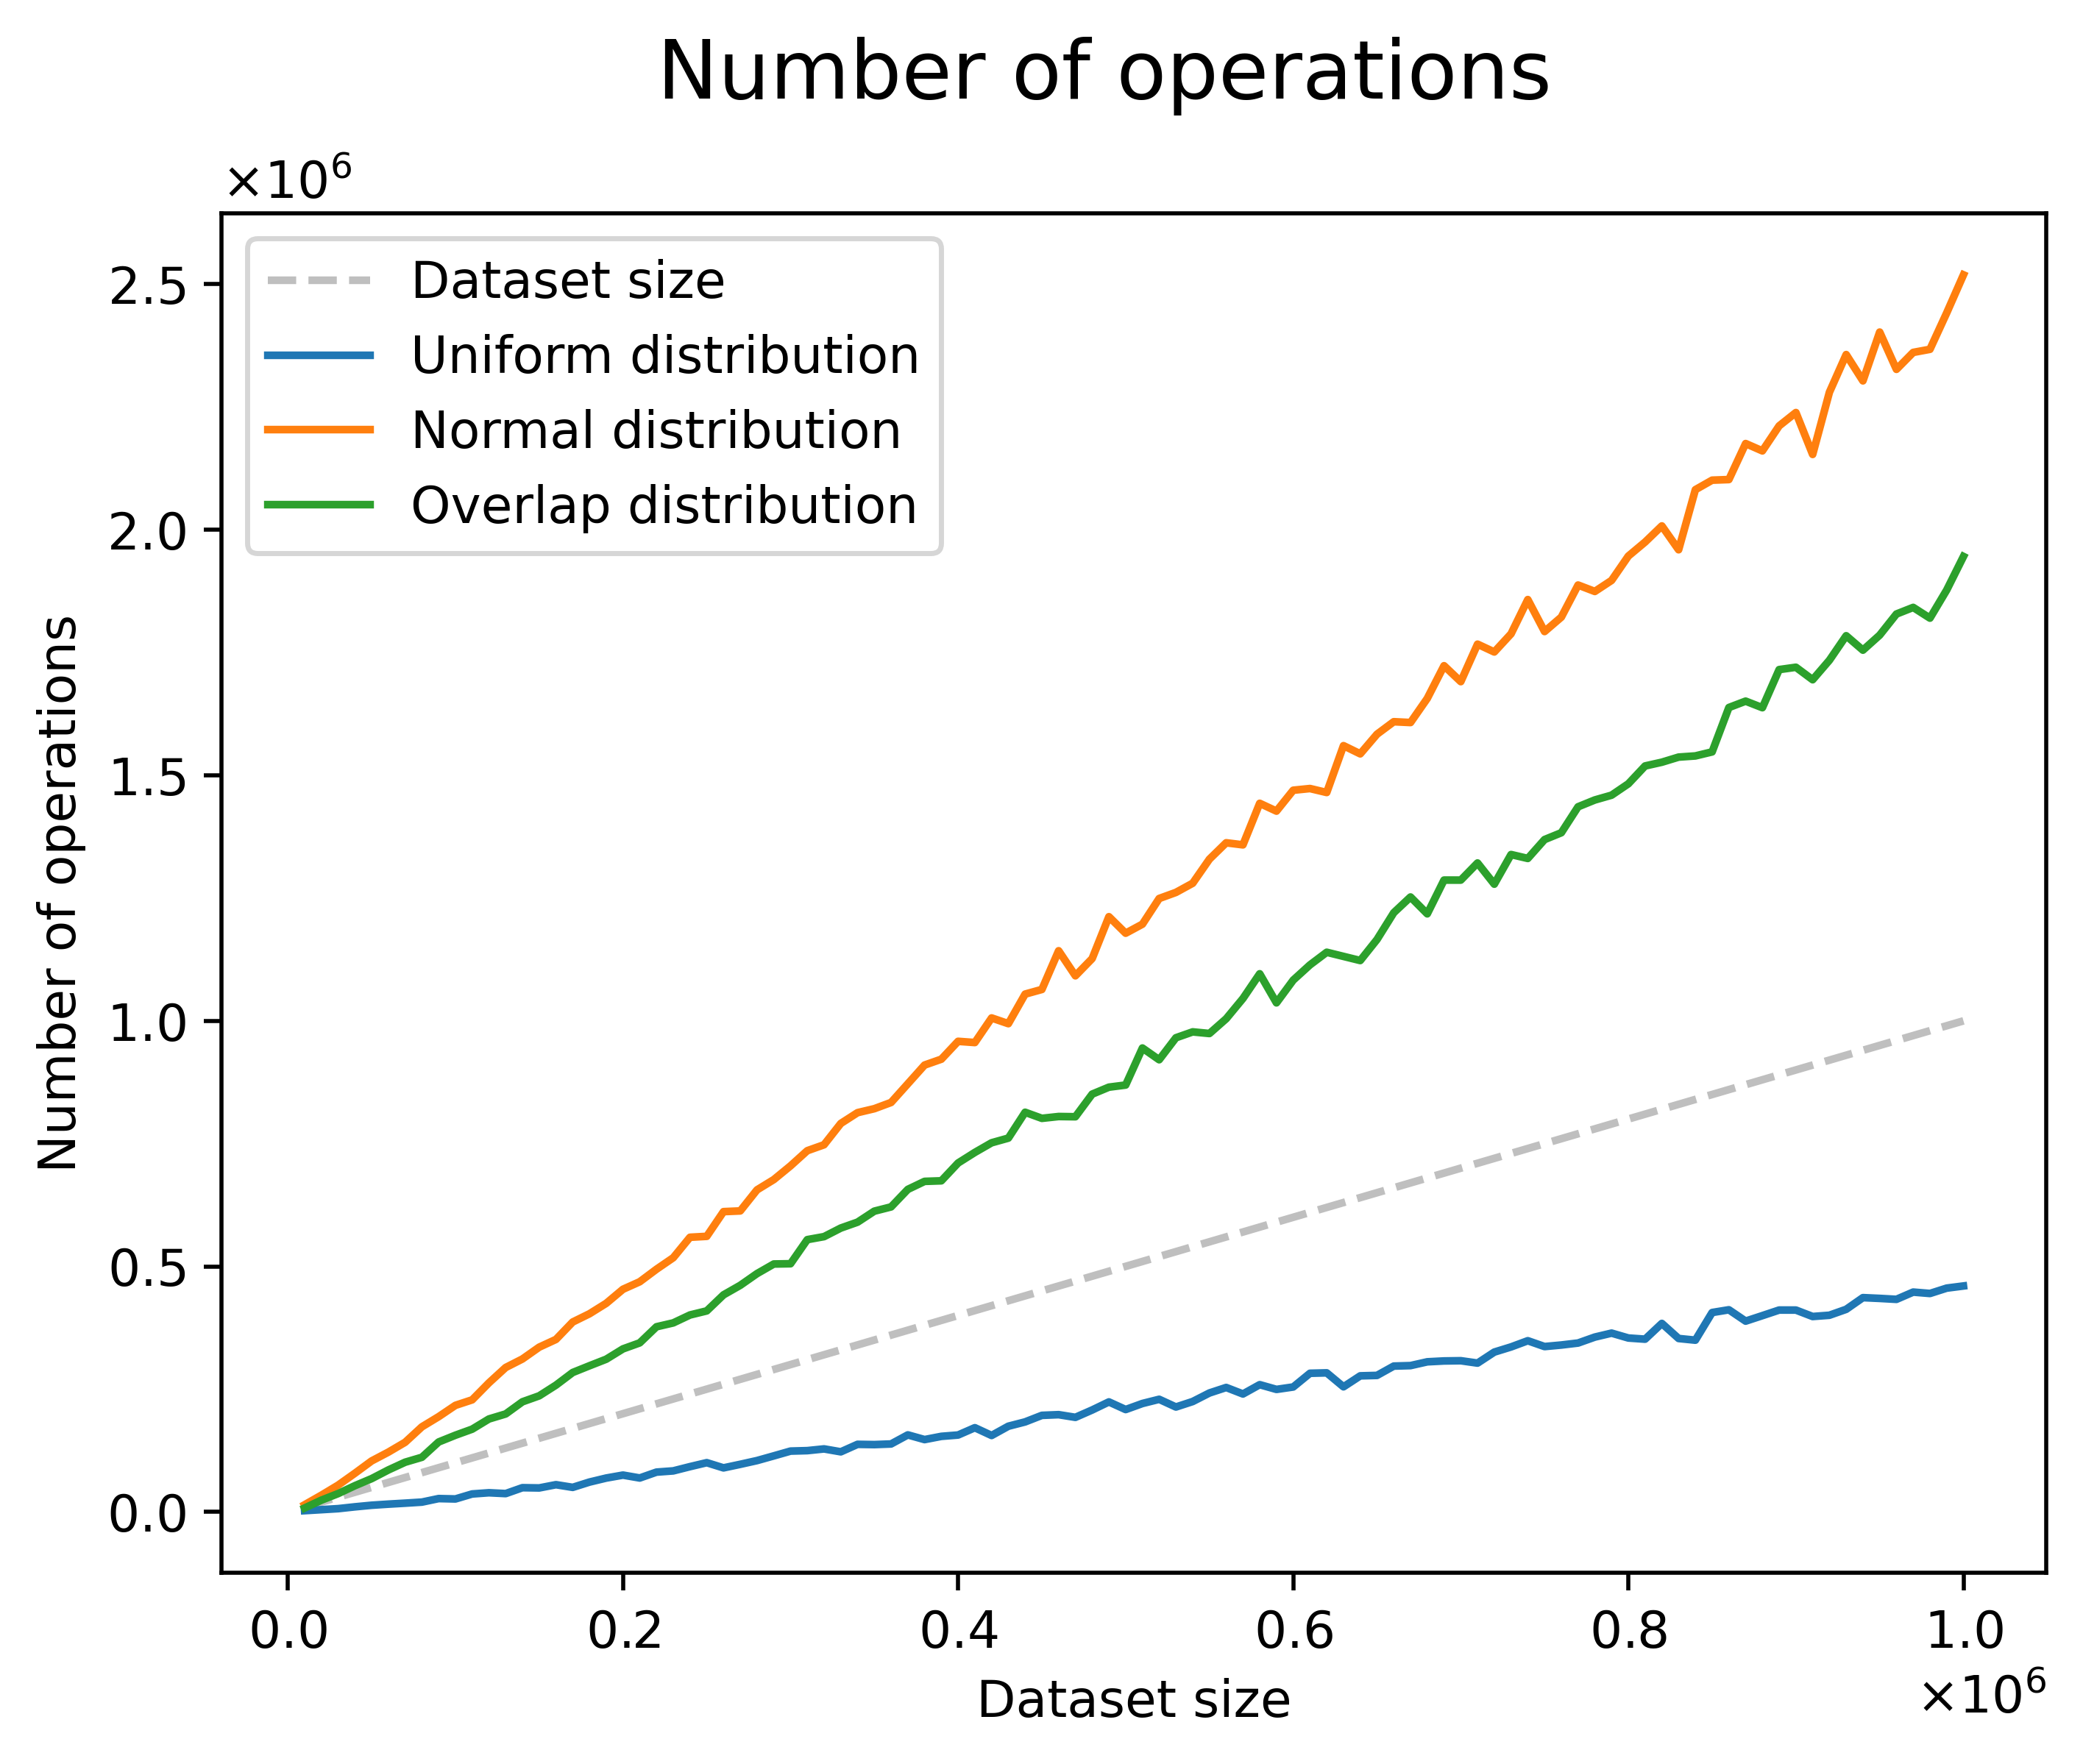
\includegraphics[width=0.5\textwidth]{figures/fig1.png}}
    \caption{Number of operations.}
    \label{fig1}
\end{figure}

\begin{figure}[htbp]
    \centerline{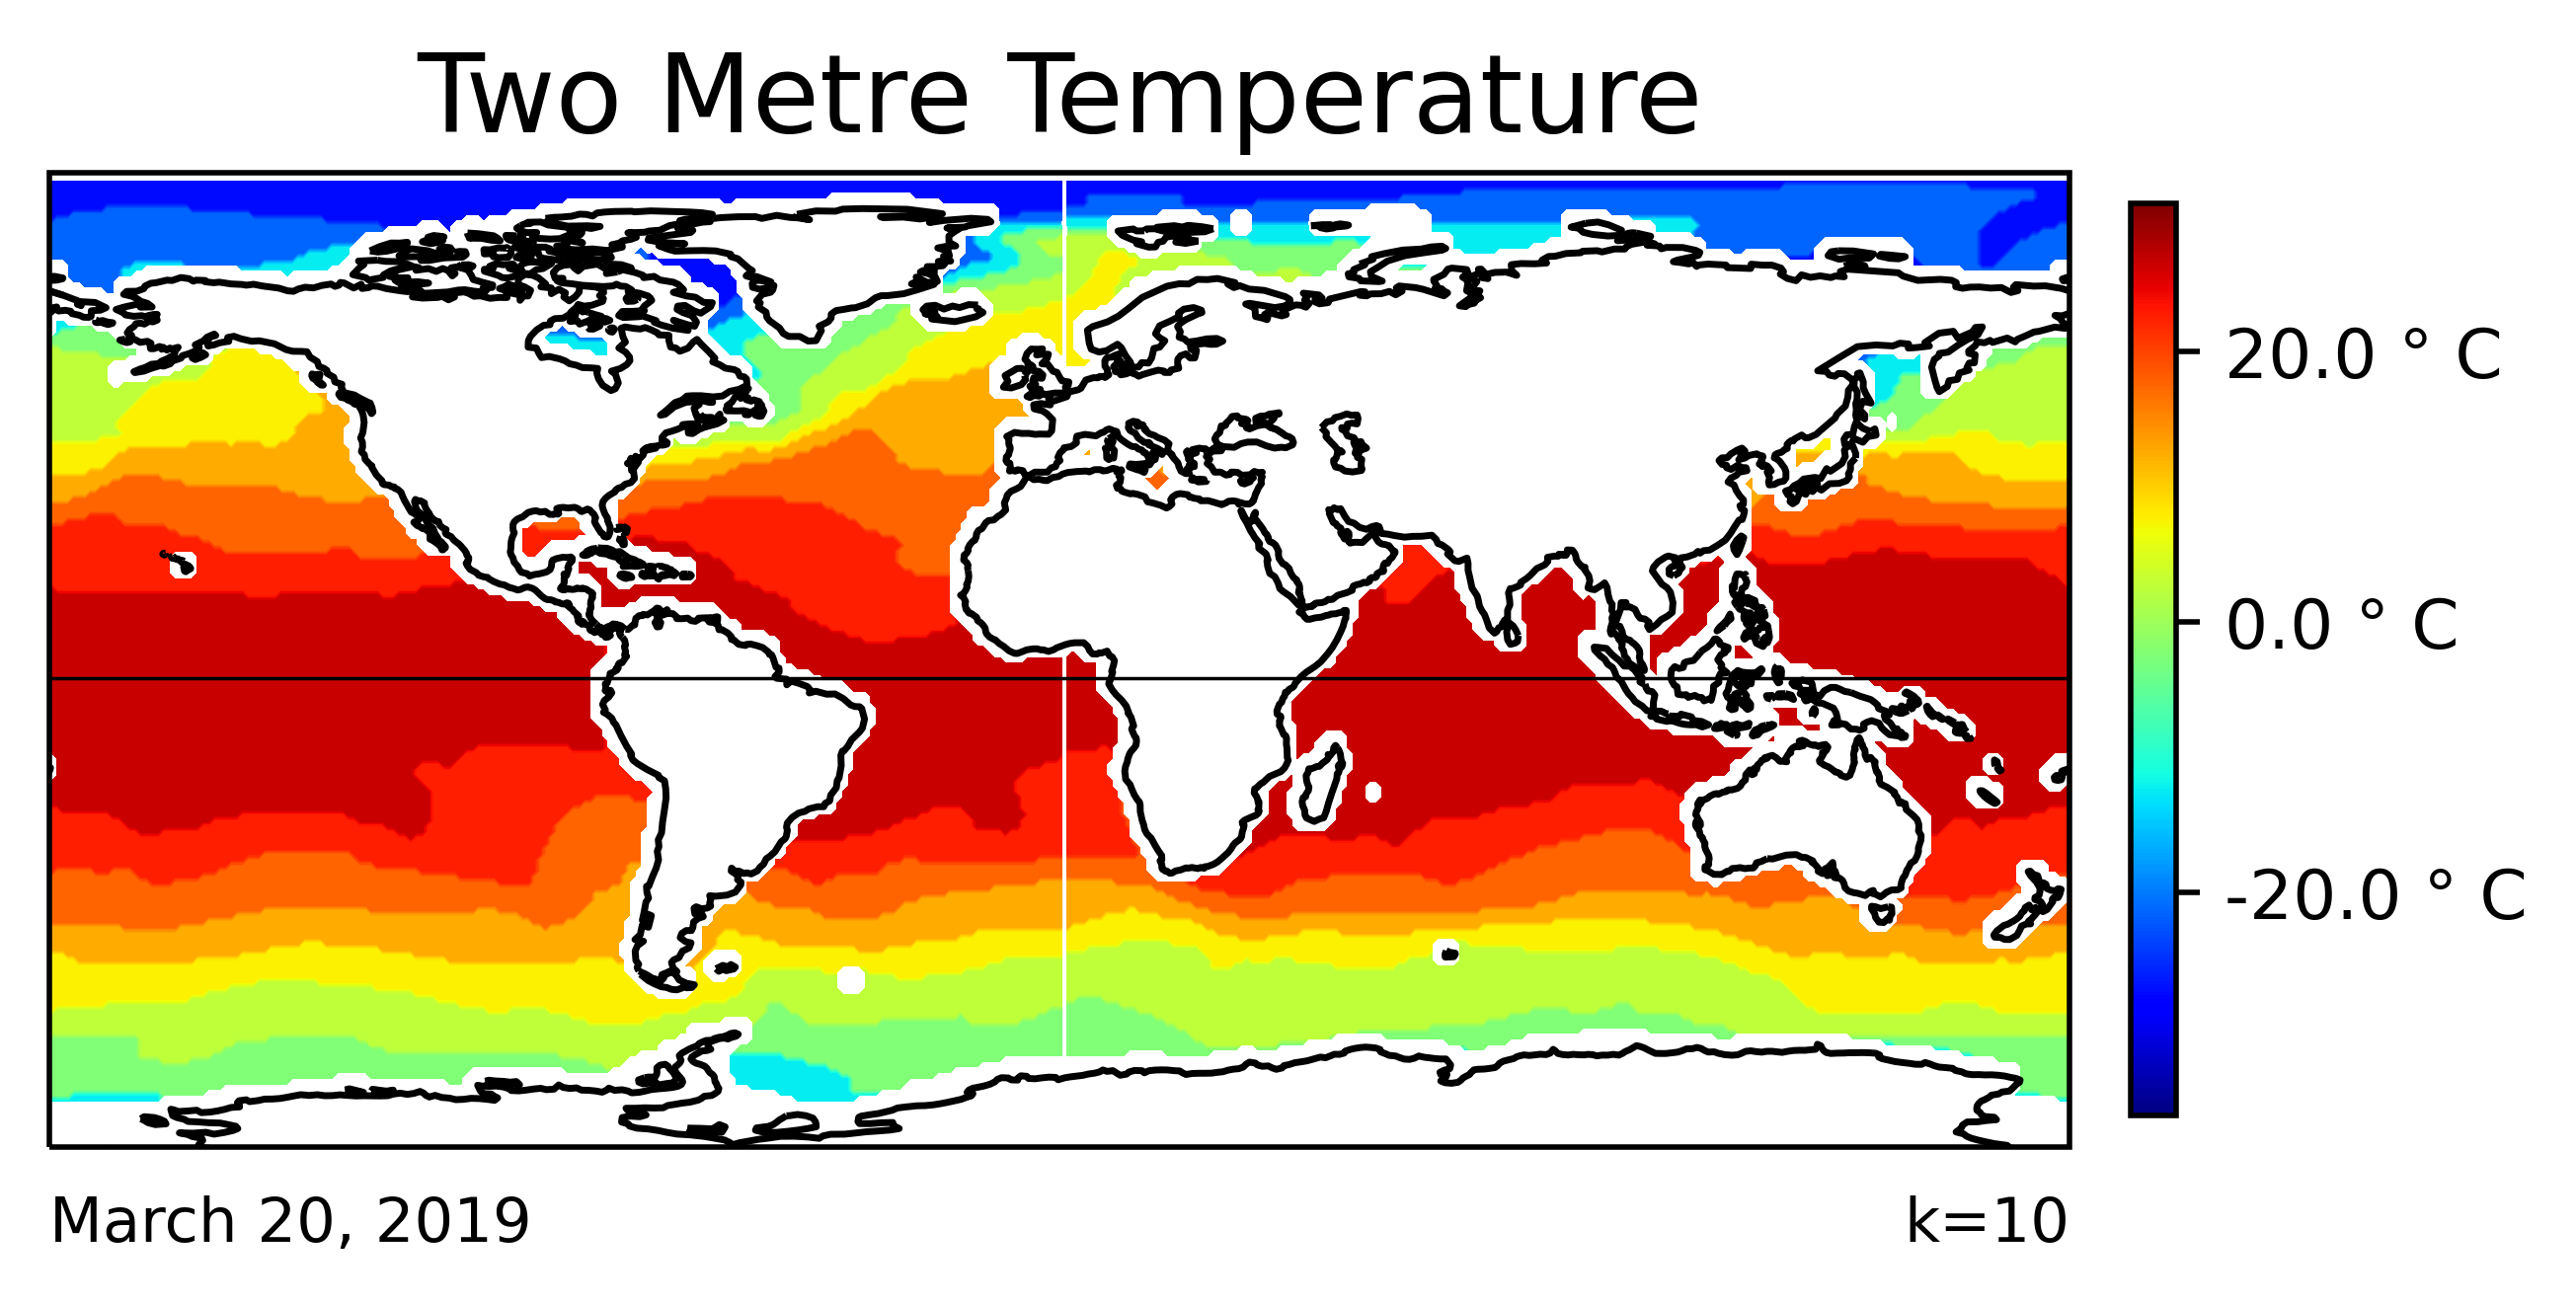
\includegraphics[width=0.5\textwidth]{figures/fig2.png}}
    \caption{Ratio of operations over dataset size.}
    \label{fig2}
\end{figure}

For the second phase of Algorithm 4 (clustering phase), the total number of operations performed is proportional to the sum of $x$ values over all iterations where $x$ is the number of positions cluster borders have moved plus $k-1$, which we denote $x_\text{sum}$. This makes the total number of operations during phase two $O(x_\text{sum})$. Figure \ref{fig1} is a plot of how $x_\text{sum}$ scales with the size of the dataset for a variety of different dataset distributions. For Figure \ref{fig1} and Figure \ref{fig2} we used three synthetic datasets: A uniform distribution, a normal distribution, and a distribution with four normal distributions overlapped, with means of 200, 800, 1200, and 1500, each with a standard deviation of 150. The data points were evenly split amongst the four normal distributions.

We can make two observations from Figure \ref{fig1}. First, $x_\text{sum}$ scales roughly linearly with the size of the dataset. Second, the slope of the ratio between $x$ and the size of the dataset changes depending on the distribution of the dataset. This slope is a big-oh constant scaling factor that could potentially be ignored, however in Figure \ref{fig2}, we show the ratio of the number of operations over the dataset size ($x_\text{sum}/n$) which appears to approximate a logarithm on the size of the dataset.

We can conclude that phase 2 of Algorithm 4, including all iterations, takes either $O(n)$ if $x_\text{sum}/n$ converges towards a constant value or $O(n \log n)$ if $x_\text{sum}/n$ follows $\log n$ time. However, since phase 1 of Algorithm 4 sorts the input dataset using a comparison-based sort, the time complexity of Algorithm 4 is $O(n \log n)$ regardless of whether phase 2 is $O(n)$ or $O(n \log n)$. This is in stark contrast to other optimized k-means algorithms which have a time complexity of $O(n^2)$ \cite{b1}.

Additionally, as with Algorithm 1, Algorithm 3 is parallelizable. As noted in the proof of correctness, the cluster dividers cannot cross each other and cause the sum and count calculations to be incorrect, even when the algorithm is executed in parallel. As such, parallelizing the algorithm is possible. If both the sorting and the clustering steps were parallelized, the total runtime for Algorithm 4 would be either $O((\log n)^2 + \frac{n}{k-1}) = O(\frac{n}{k})$ or $O((\log n)^2 + \frac{n}{k-1} \log n) = O(\frac{n}{k} \log n)$, depending on the true complexity of phase 2 \cite{b6}.

To summarize our results, Algorithm 4 has a time complexity of $O(n \log n)$ when executed sequentially and a time complexity of at most $O(\frac{n}{k} \log n)$ when executed in parallel.

\section{Visualization}

\subsection{Dataset}

So far we have applied our f-clustering algorithm to various artificial datasets but we now apply it to a real-world dataset containing oceanographic hydrological and marine meteorological data \cite{b4}. We then visualize the results in two different formats to make the data easier to interpret. Ocean and atmosphere data requires data preprocessing, conversion, and manipulation to properly understand it due to its vast, complex, and high volume nature \cite{b4}. We use the ERA5 global climate and weather dataset which contains hourly data on single levels from 1979 to present. ERA5 uses reanalysis and data assimilation techniques which combine the use of model data and observations to create a complete dataset with pre-interpolated data points aligned with a regular latitude/longitude grid in 0.25º intervals. For our visualizations, our dataset contains the sea surface temperature, mean sea level pressure (globally), atmospheric temperature two metres above the surface of the earth, and land-sea mask data at hour 00 for every day in the year 2019. This results in 1,440 data points across the longitudinal range of [0,360] and 720 data points across the latitudinal range of [0,180] for a total of 1,036,800 data points per variable per day. This totals 378,432,000 data points for the entire year per variable or 1,513,728,000 when considering all variables. With four variables, the number of data points in the dataset is incredibly large and therefore difficult to process. We perform the data pre-processing in parallel to greatly reduce the execution time required to process the data.

\subsection{Data Pre-processing}

We perform three data pre-processing algorithms to the original dataset. First, to increase the speed of our f-clustering algorithm without significant loss of data precision, we take the original dataset and significantly reduce its size. This is done by iterating through every data point located at an integer latitude/longitude coordinate and calculating an averaged data point using the grid of data points located four data points above and to the right of the averaged data point. Running this averaging algorithm on each of the variables from the original dataset excluding the sea-land mask variable reduces a variable's size from 1,036,800 to 64,800 data points per day without losing significant amounts of precision. This leads to a total reduction of 1,135,296,000 to 70,956,000 data points. Second, because our two metre atmosphere temperature and mean sea level pressure variables contain data covering the entire globe (including land) we use the land-sea mask variable to remove any data points that were measured above land. This helps keep the focus of our visualization on oceanic data. Last, we remove any averaged data points that contain one or more masked values in their averaging calculation. We parallelize these data pre-processing algorithms which greatly reduces the execution time of the data pre-processing stage.

\subsection{Visualizations}

\begin{figure}[htbp]
    \centerline{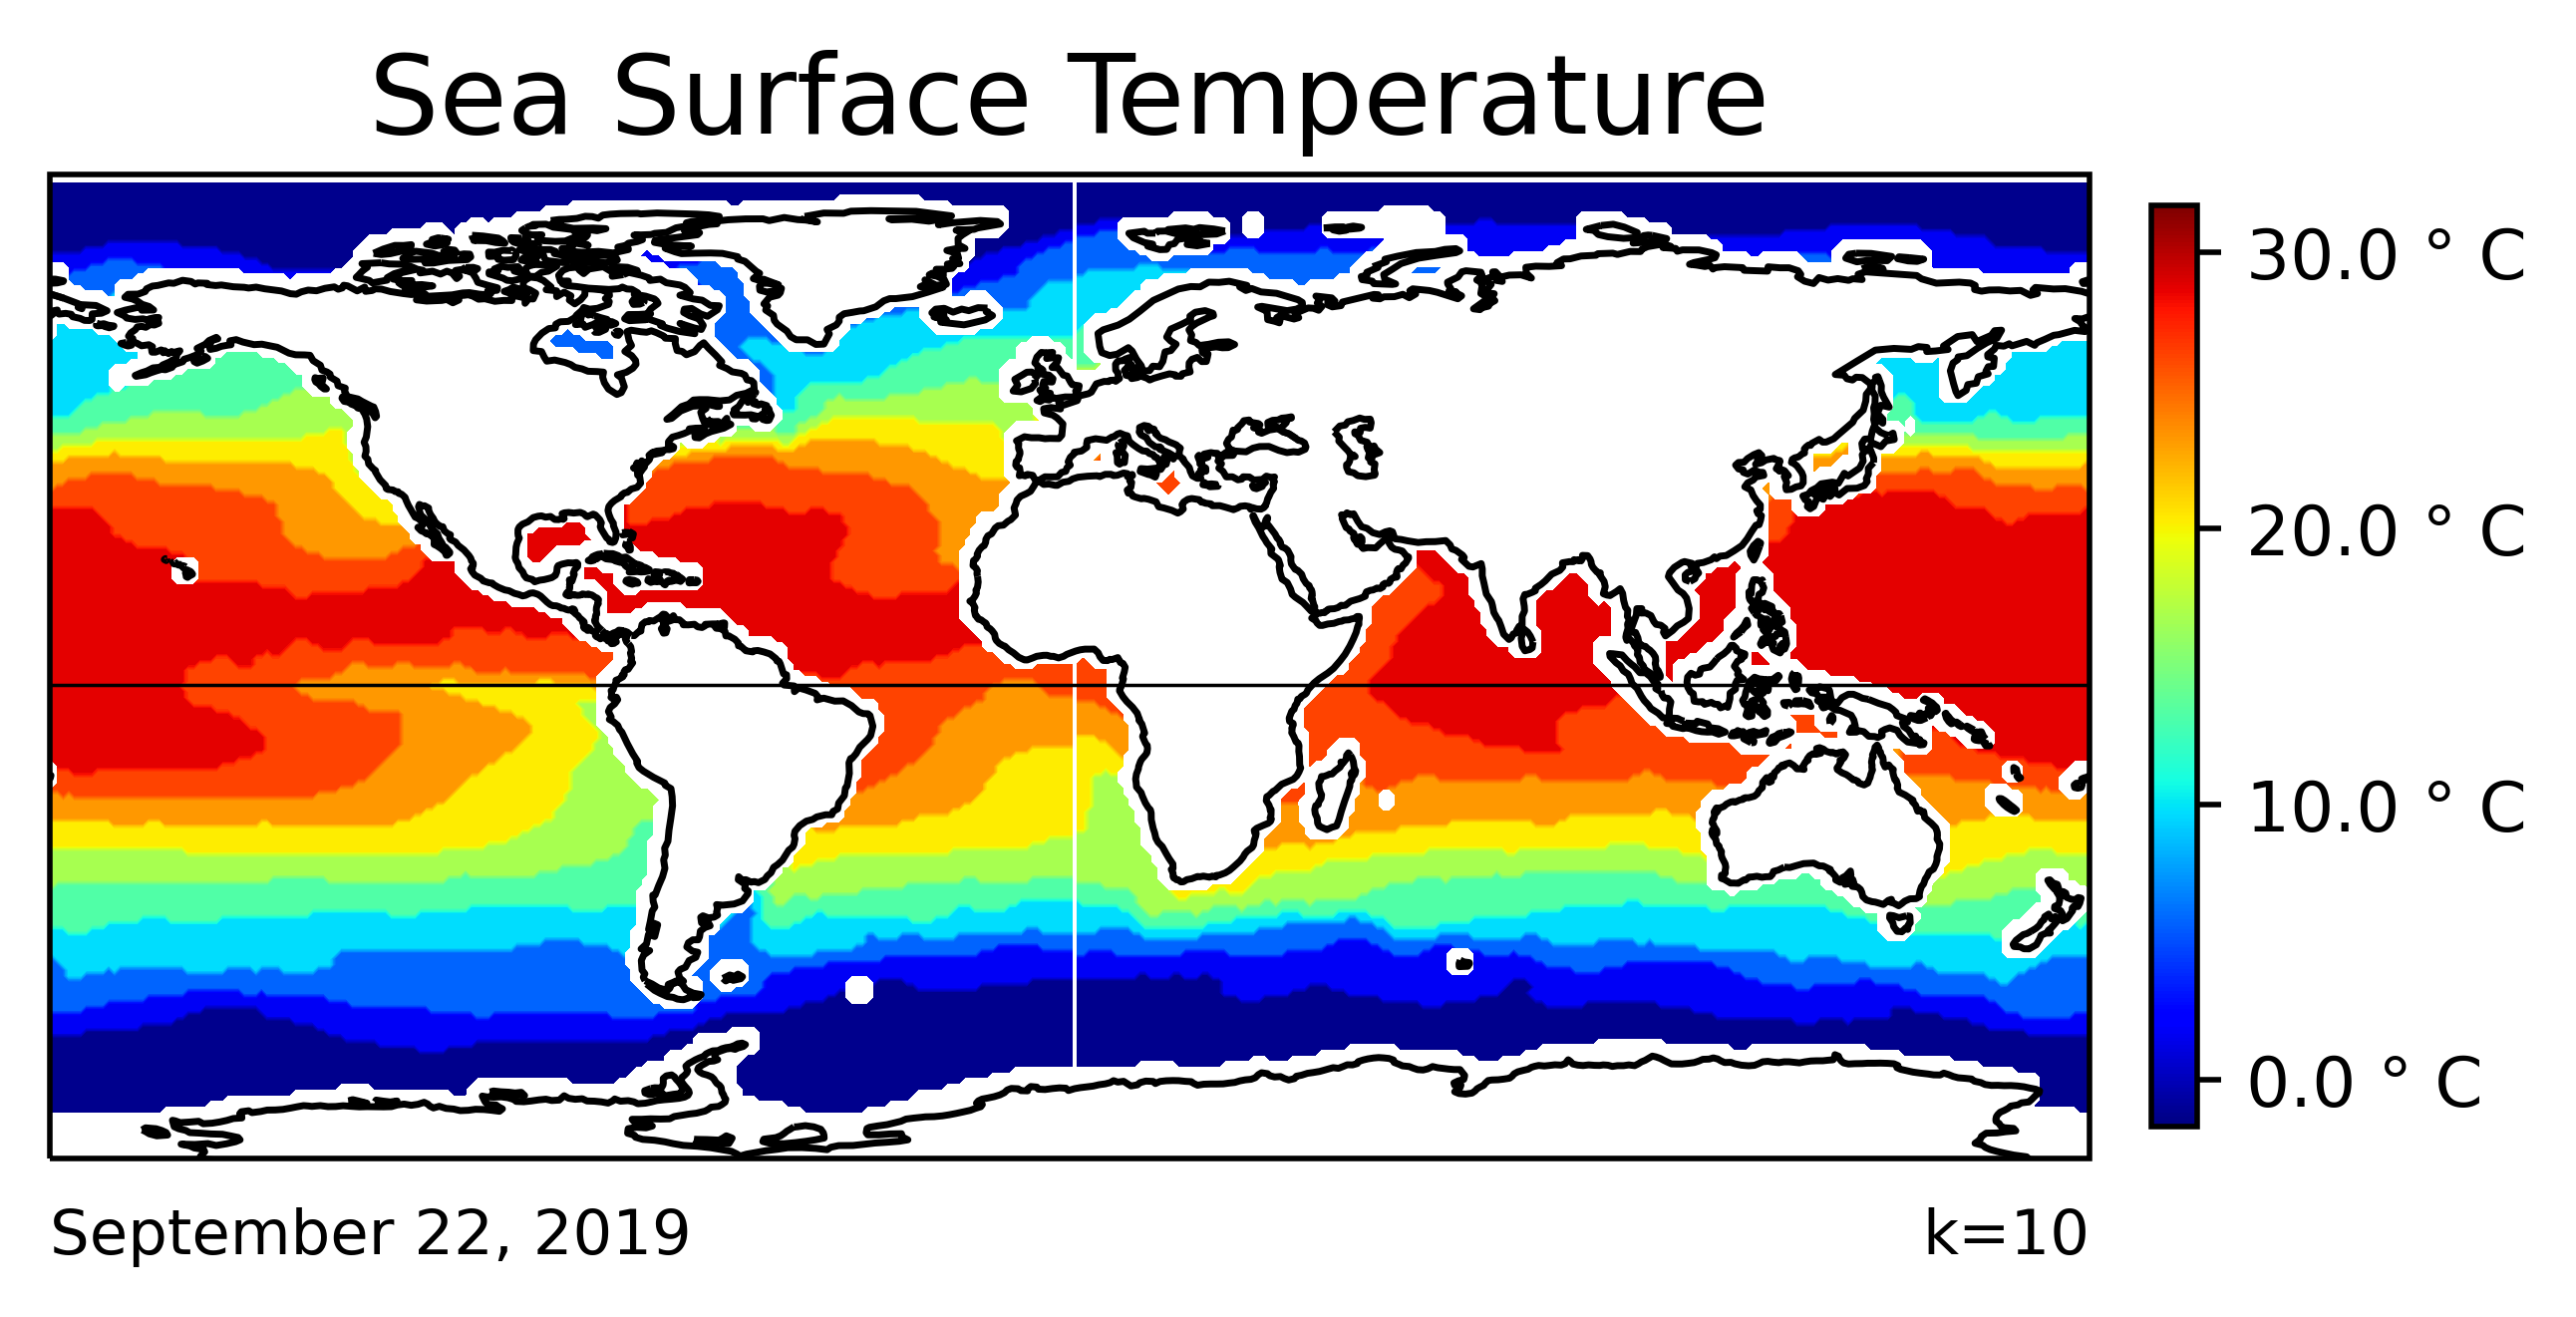
\includegraphics[width=0.5\textwidth]{figures/fig3.png}}
    \caption{Sea Surface Temperature on March 20th 2019.}
    \label{fig3}
\end{figure}
\begin{figure}[htbp]
    \centerline{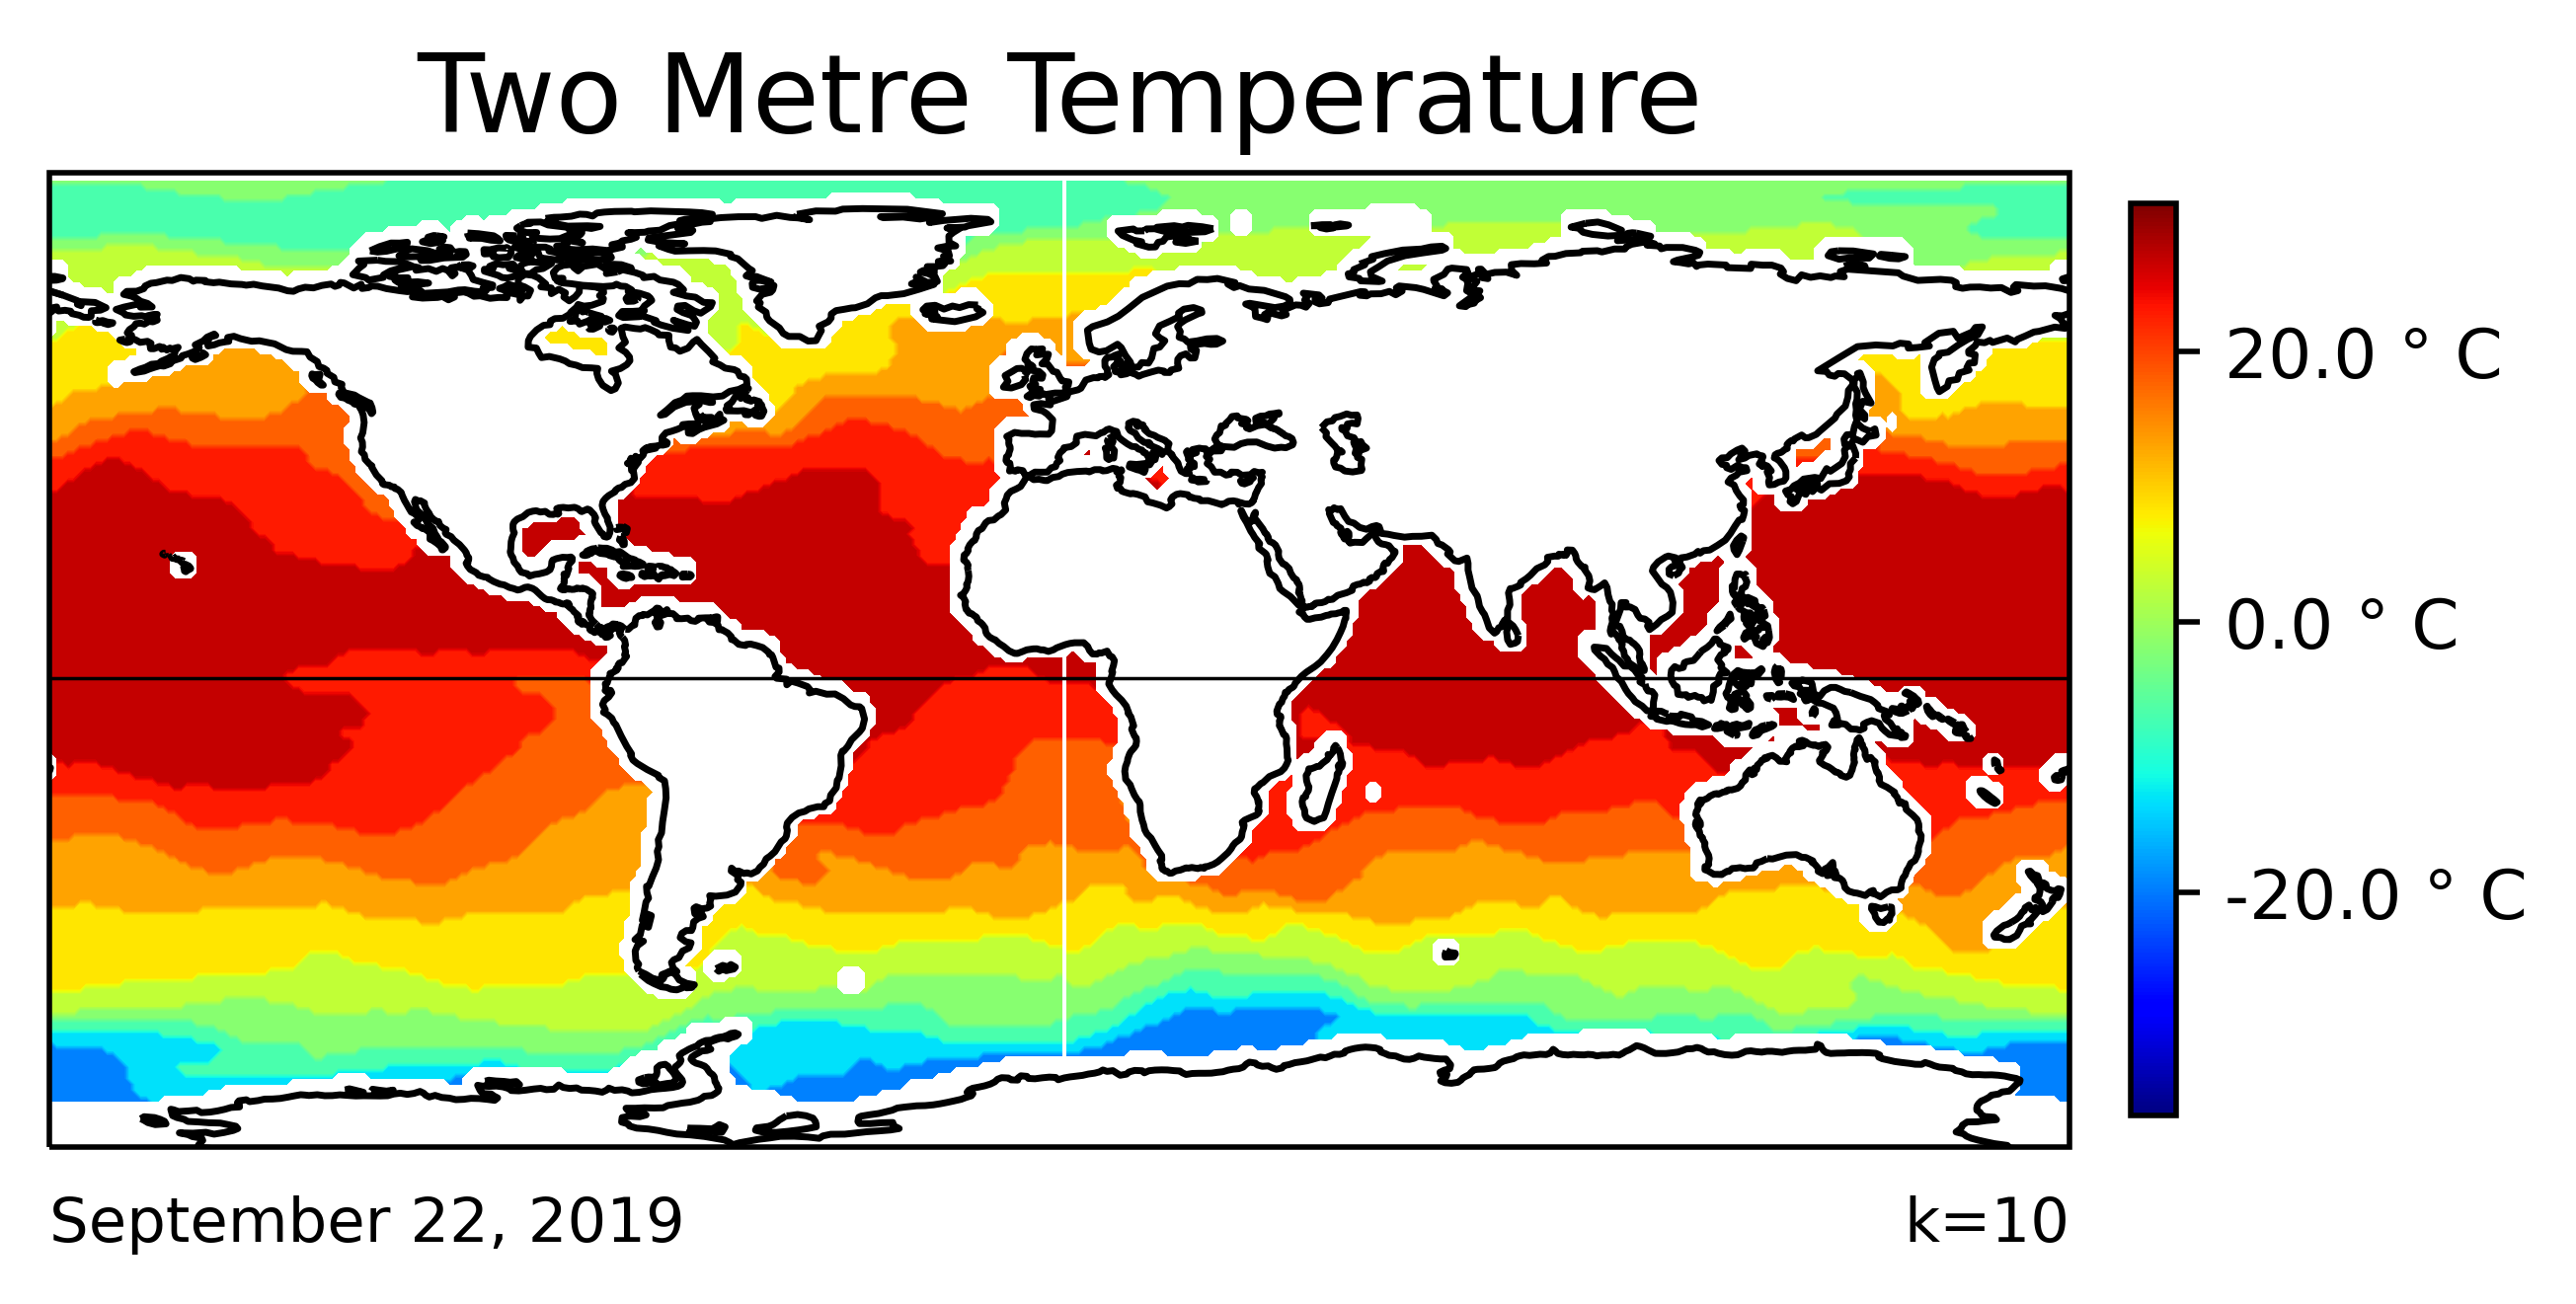
\includegraphics[width=0.5\textwidth]{figures/fig4.png}}
    \caption{Two Metre Atmosphere Temperature on March 20th 2019.}
    \label{fig4}
\end{figure}
\begin{figure}[htbp]
    \centerline{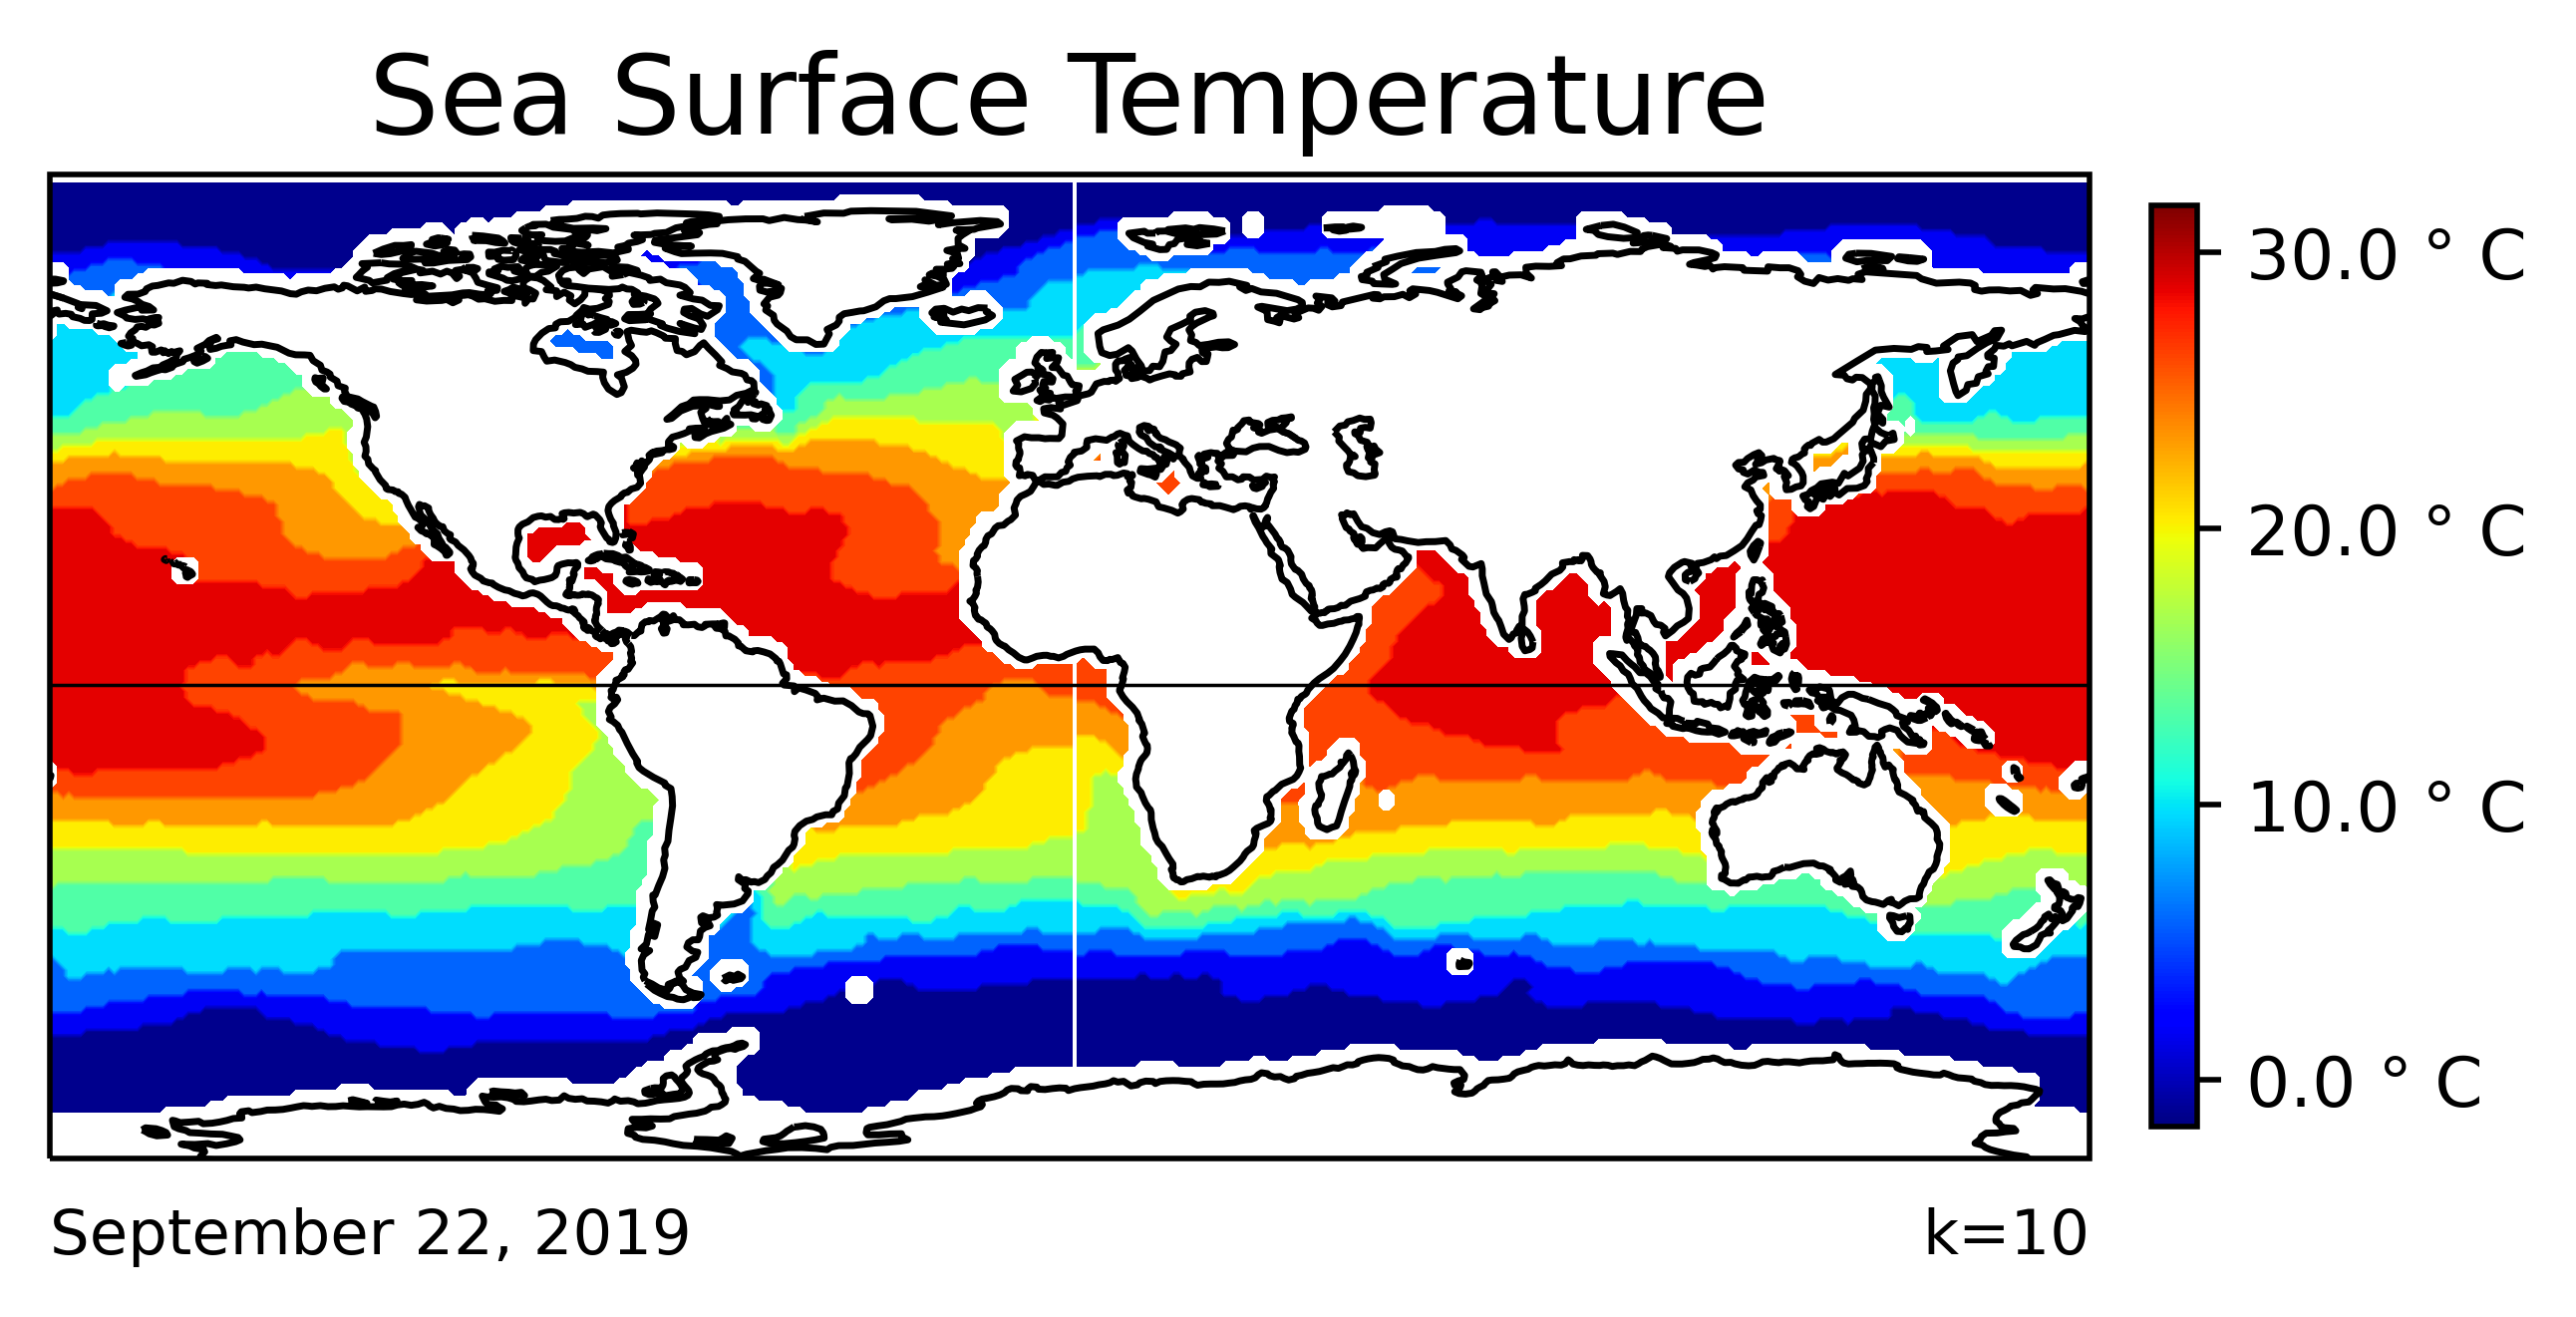
\includegraphics[width=0.5\textwidth]{figures/fig5.png}}
    \caption{Sea Surface Temperature on September 22nd 2019.}
    \label{fig5}
\end{figure}
\begin{figure}[htbp]
    \centerline{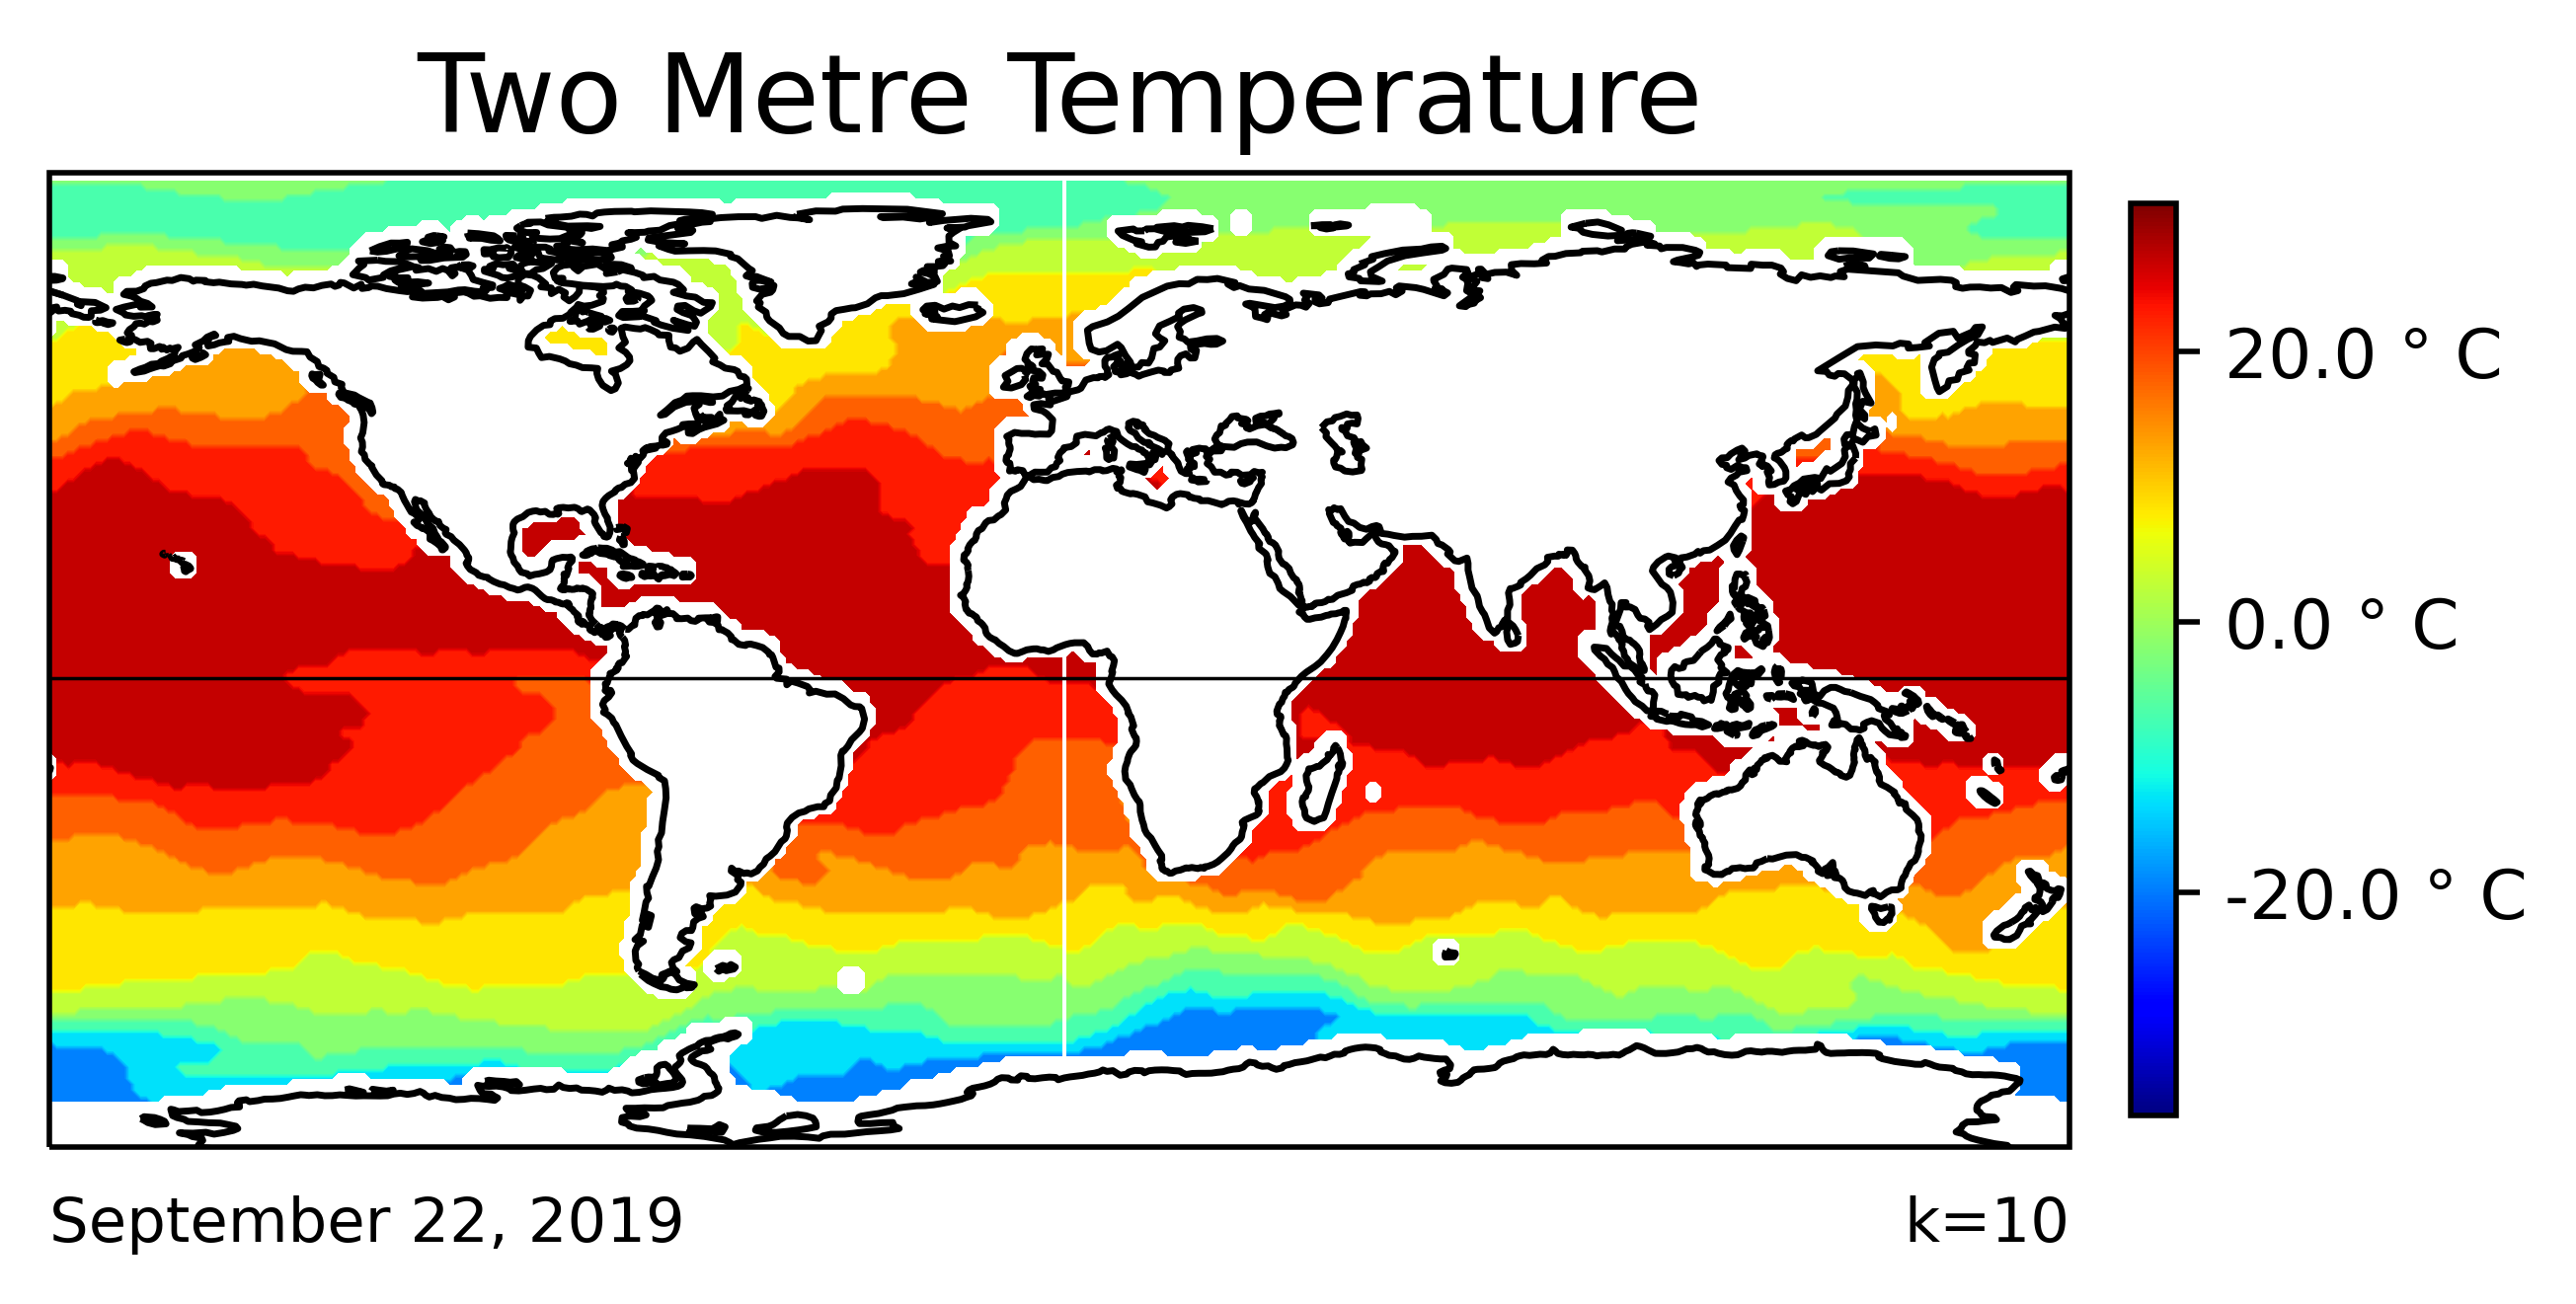
\includegraphics[width=0.5\textwidth]{figures/fig6.png}}
    \caption{Two Metre Atmosphere Temperature on September 22nd 2019.}
    \label{fig6}
\end{figure}

We created two different types of visualizations to represent the clustered data. The first visualization plots each cluster on an equirectangular projection of the Earth. Each cluster is coloured based on the value of its centroid. The second visualization is a discrete stepped line graph representing the changes in the values of the variable on the y-axis over a single line of latitude of the earth, from the South Pole to the North Pole. Each cluster appears as a step in the line which is helpful for understanding which latitude clusters of similar values are located on the earth. For each variable, we generated a line graph and a map plot for each day of the year. We then created an animated video for each variable and visualization type. This provides an easy way to visually represent any changing trends in the data throughout the year 2019.

Using the visualizations we created, we can gather useful information from the original dataset. When looking at the map plots of sea surface temperature and two metre atmosphere temperature we can see that the regions close to the equator have a higher temperature than the regions closer to the poles, as expected. Furthermore, we can see the distribution of similar data points by observing the size of each cluster. We see in Figure \ref{fig4} that a large portion of the earth around the equator has a similar air temperature of around 25º Celsius. This is in contrast to the air temperature in the North Pole region that is sub 20ª Celsius that covers much less of the map. We can see from observing Figure \ref{fig3} that the sea surface temperature similarly has cold regions at both poles while the two metre air temperature in Figure \ref{fig4} is only that cold at the North Pole.

Another key observation we can make is how the clusters change over time throughout the year. When comparing Figure \ref{fig4} and Figure \ref{fig6} we can see that on March 20th, 2019 in Figure \ref{fig4} the regions near the North Pole are much colder than the same region in Figure \ref{fig6} on September 22nd, 2019. Similarly, in Figure \ref{fig4} the temperatures directly above Antarctica are warmer than the same region in Figure \ref{fig6}. When considering the cluster with the hottest temperatures, we see that it’s position on the map in Figure \ref{fig4} moves from just below the equator to above the equator in Figure \ref{fig6}. A similar effect can also be seen in Figure \ref{fig3} and Figure \ref{fig5} where the warmest water is located roughly just below the equator in Figure \ref{fig3} and slightly above the equator in Figure \ref{fig5}.

\begin{figure}[htbp]
    \centerline{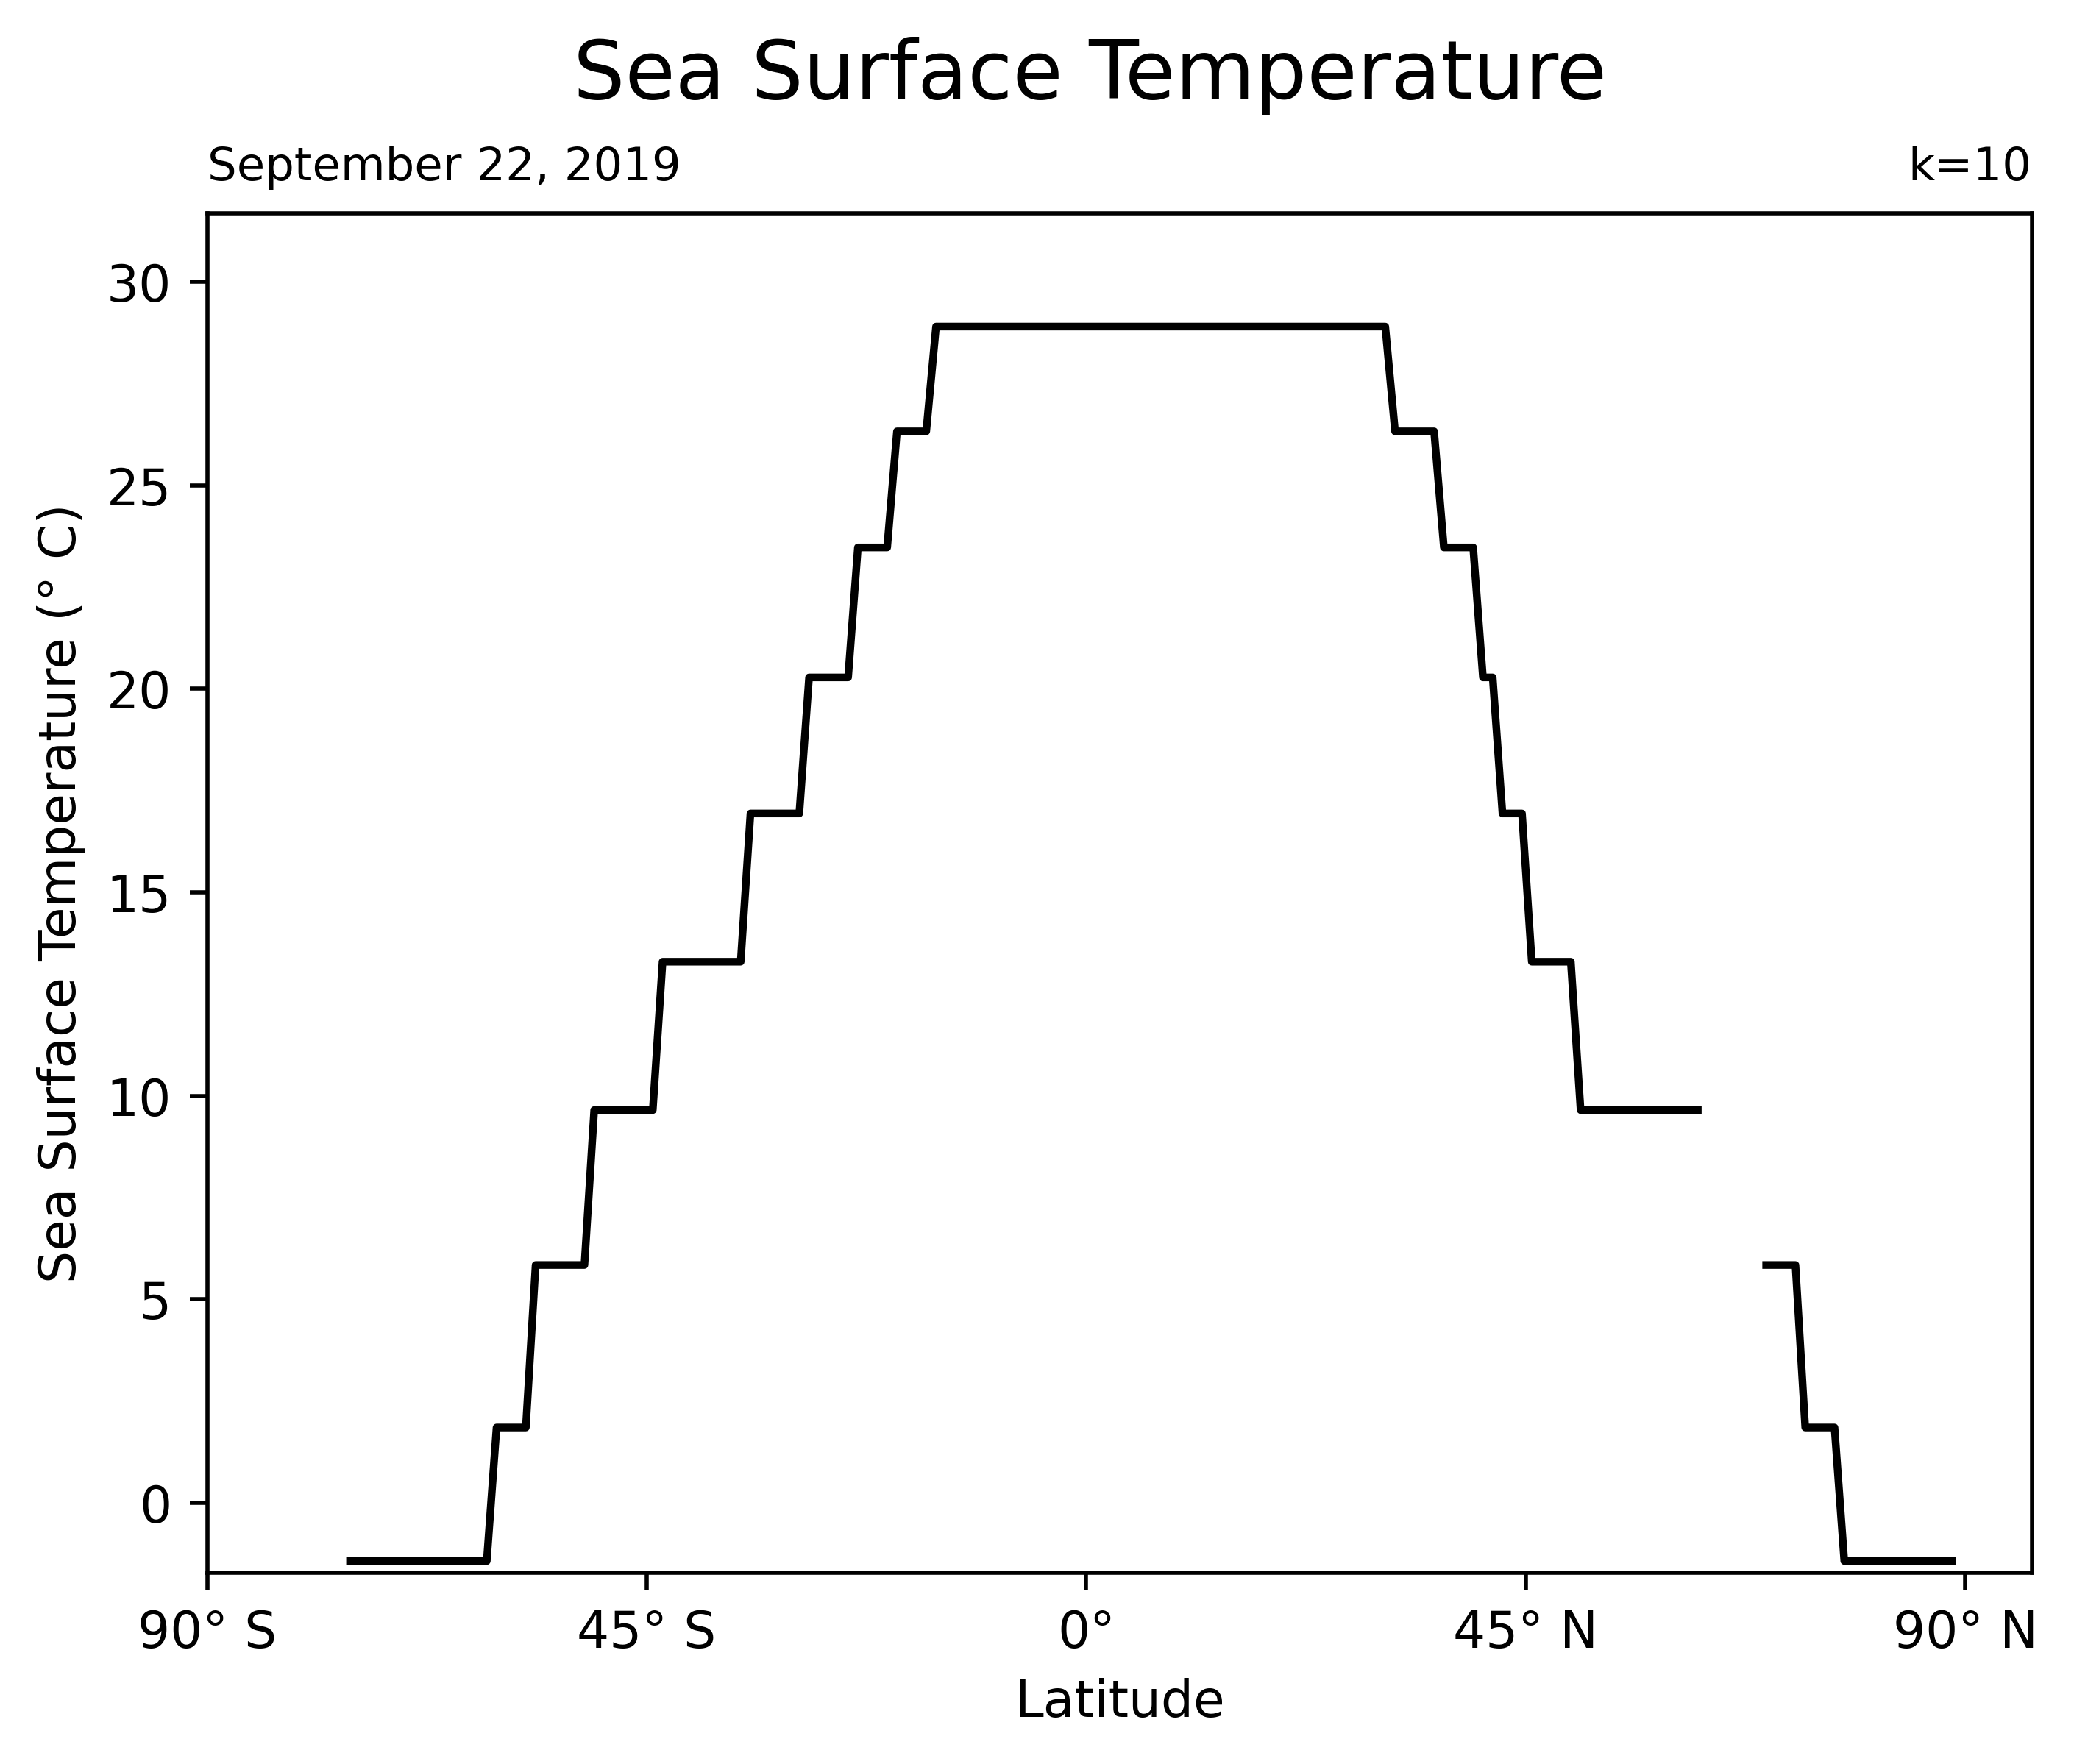
\includegraphics[width=0.5\textwidth]{figures/fig7.png}}
    \caption{Sea Surface Temperature on March 20th 2019.}
    \label{fig7}
\end{figure}
\begin{figure}[htbp]
    \centerline{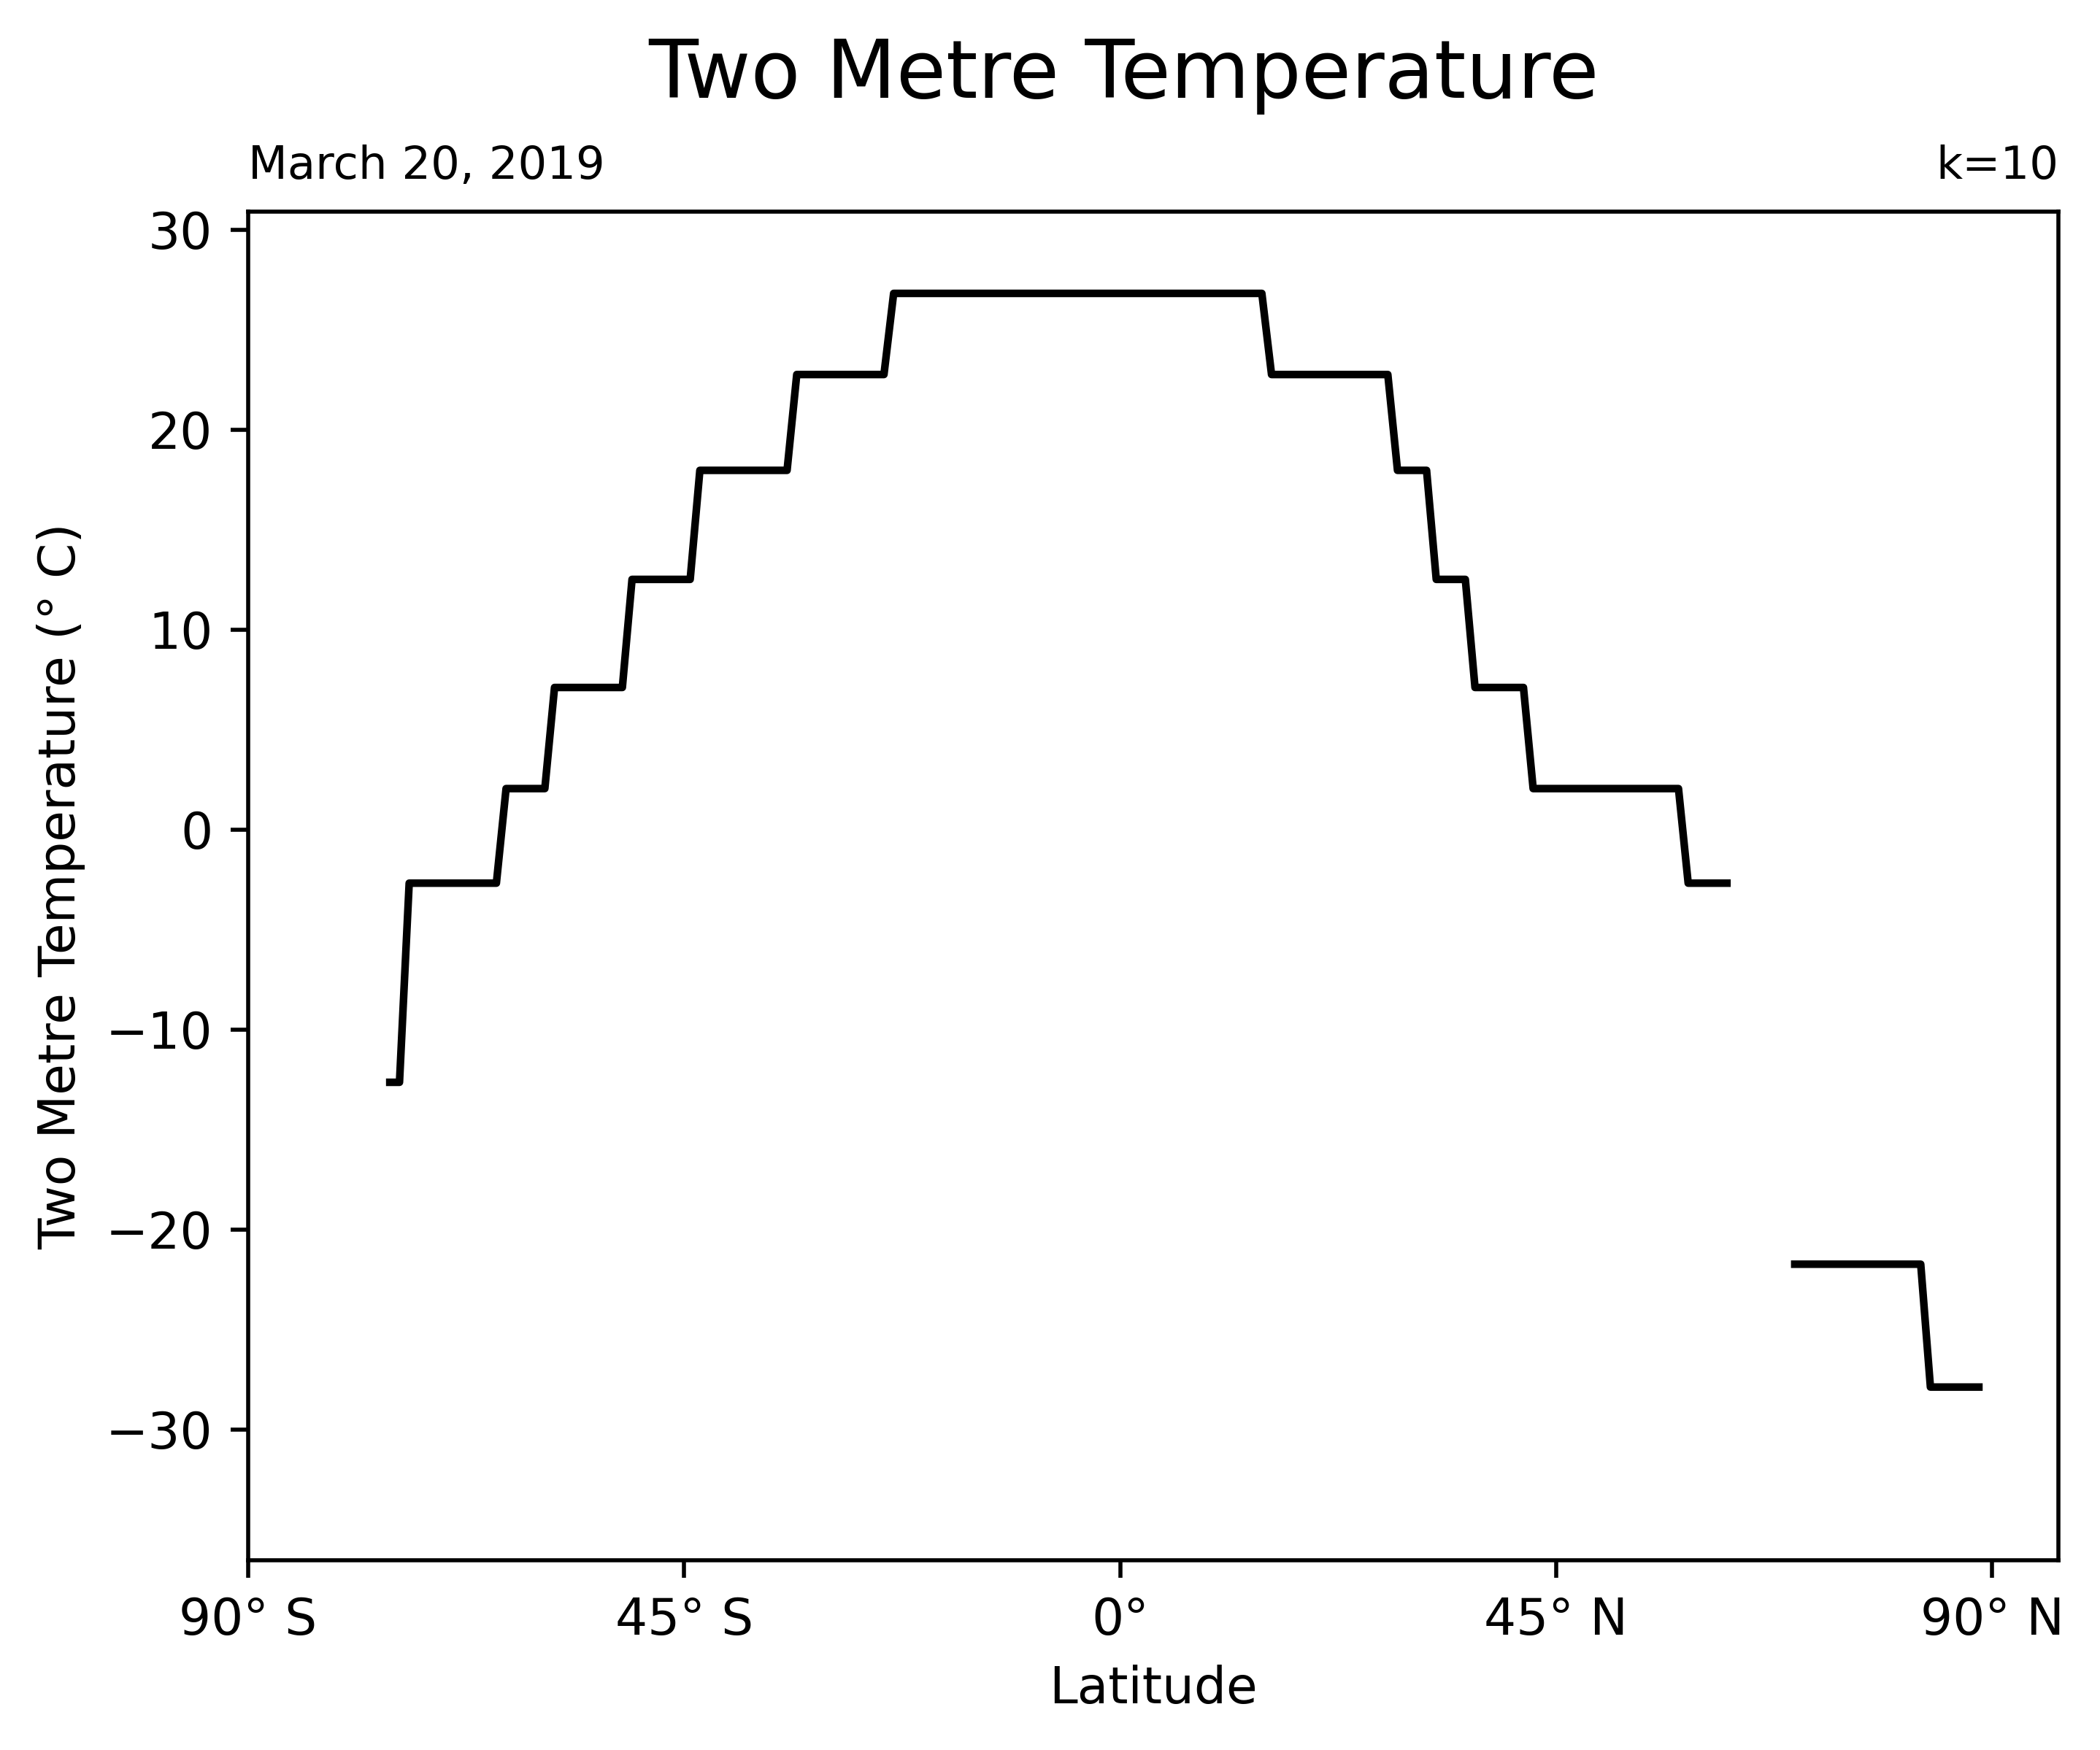
\includegraphics[width=0.5\textwidth]{figures/fig8.png}}
    \caption{Two Metre Atmosphere Temperature on March 20th 2019.}
    \label{fig8}
\end{figure}
\begin{figure}[htbp]
    \centerline{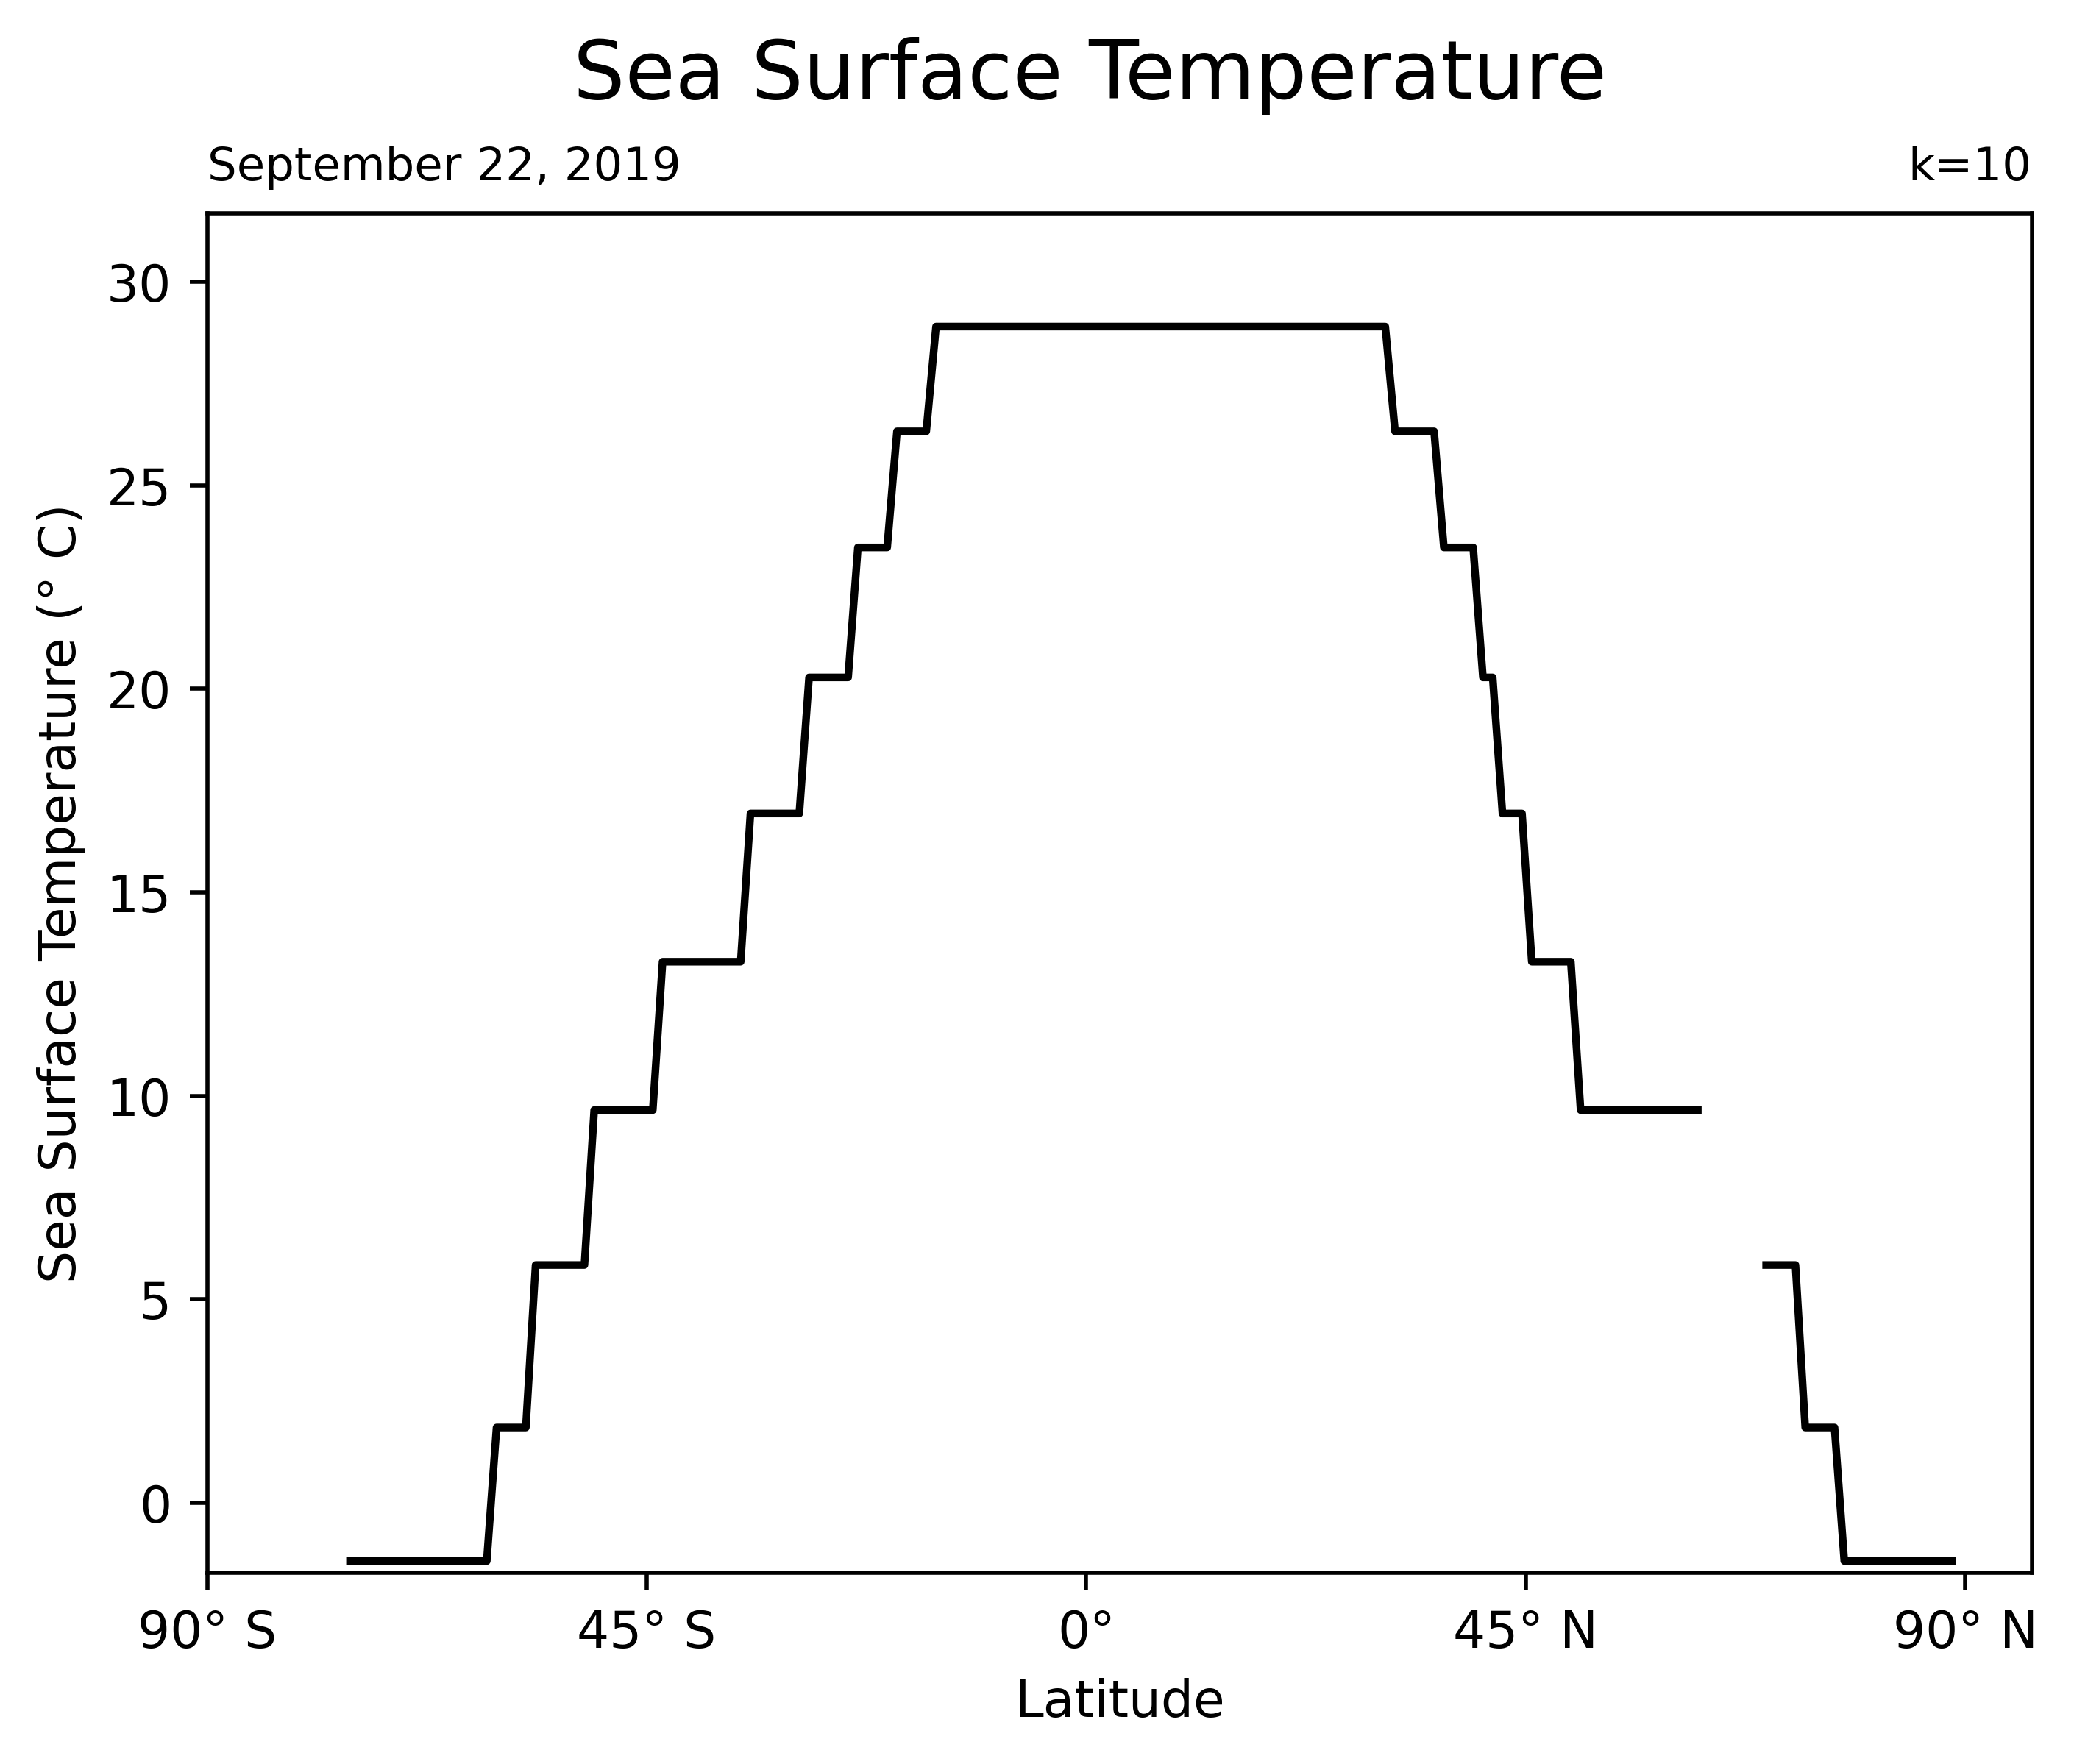
\includegraphics[width=0.5\textwidth]{figures/fig9.png}}
    \caption{Sea Surface Temperature on September 22nd 2019.}
    \label{fig9}
\end{figure}
\begin{figure}[htbp]
    \centerline{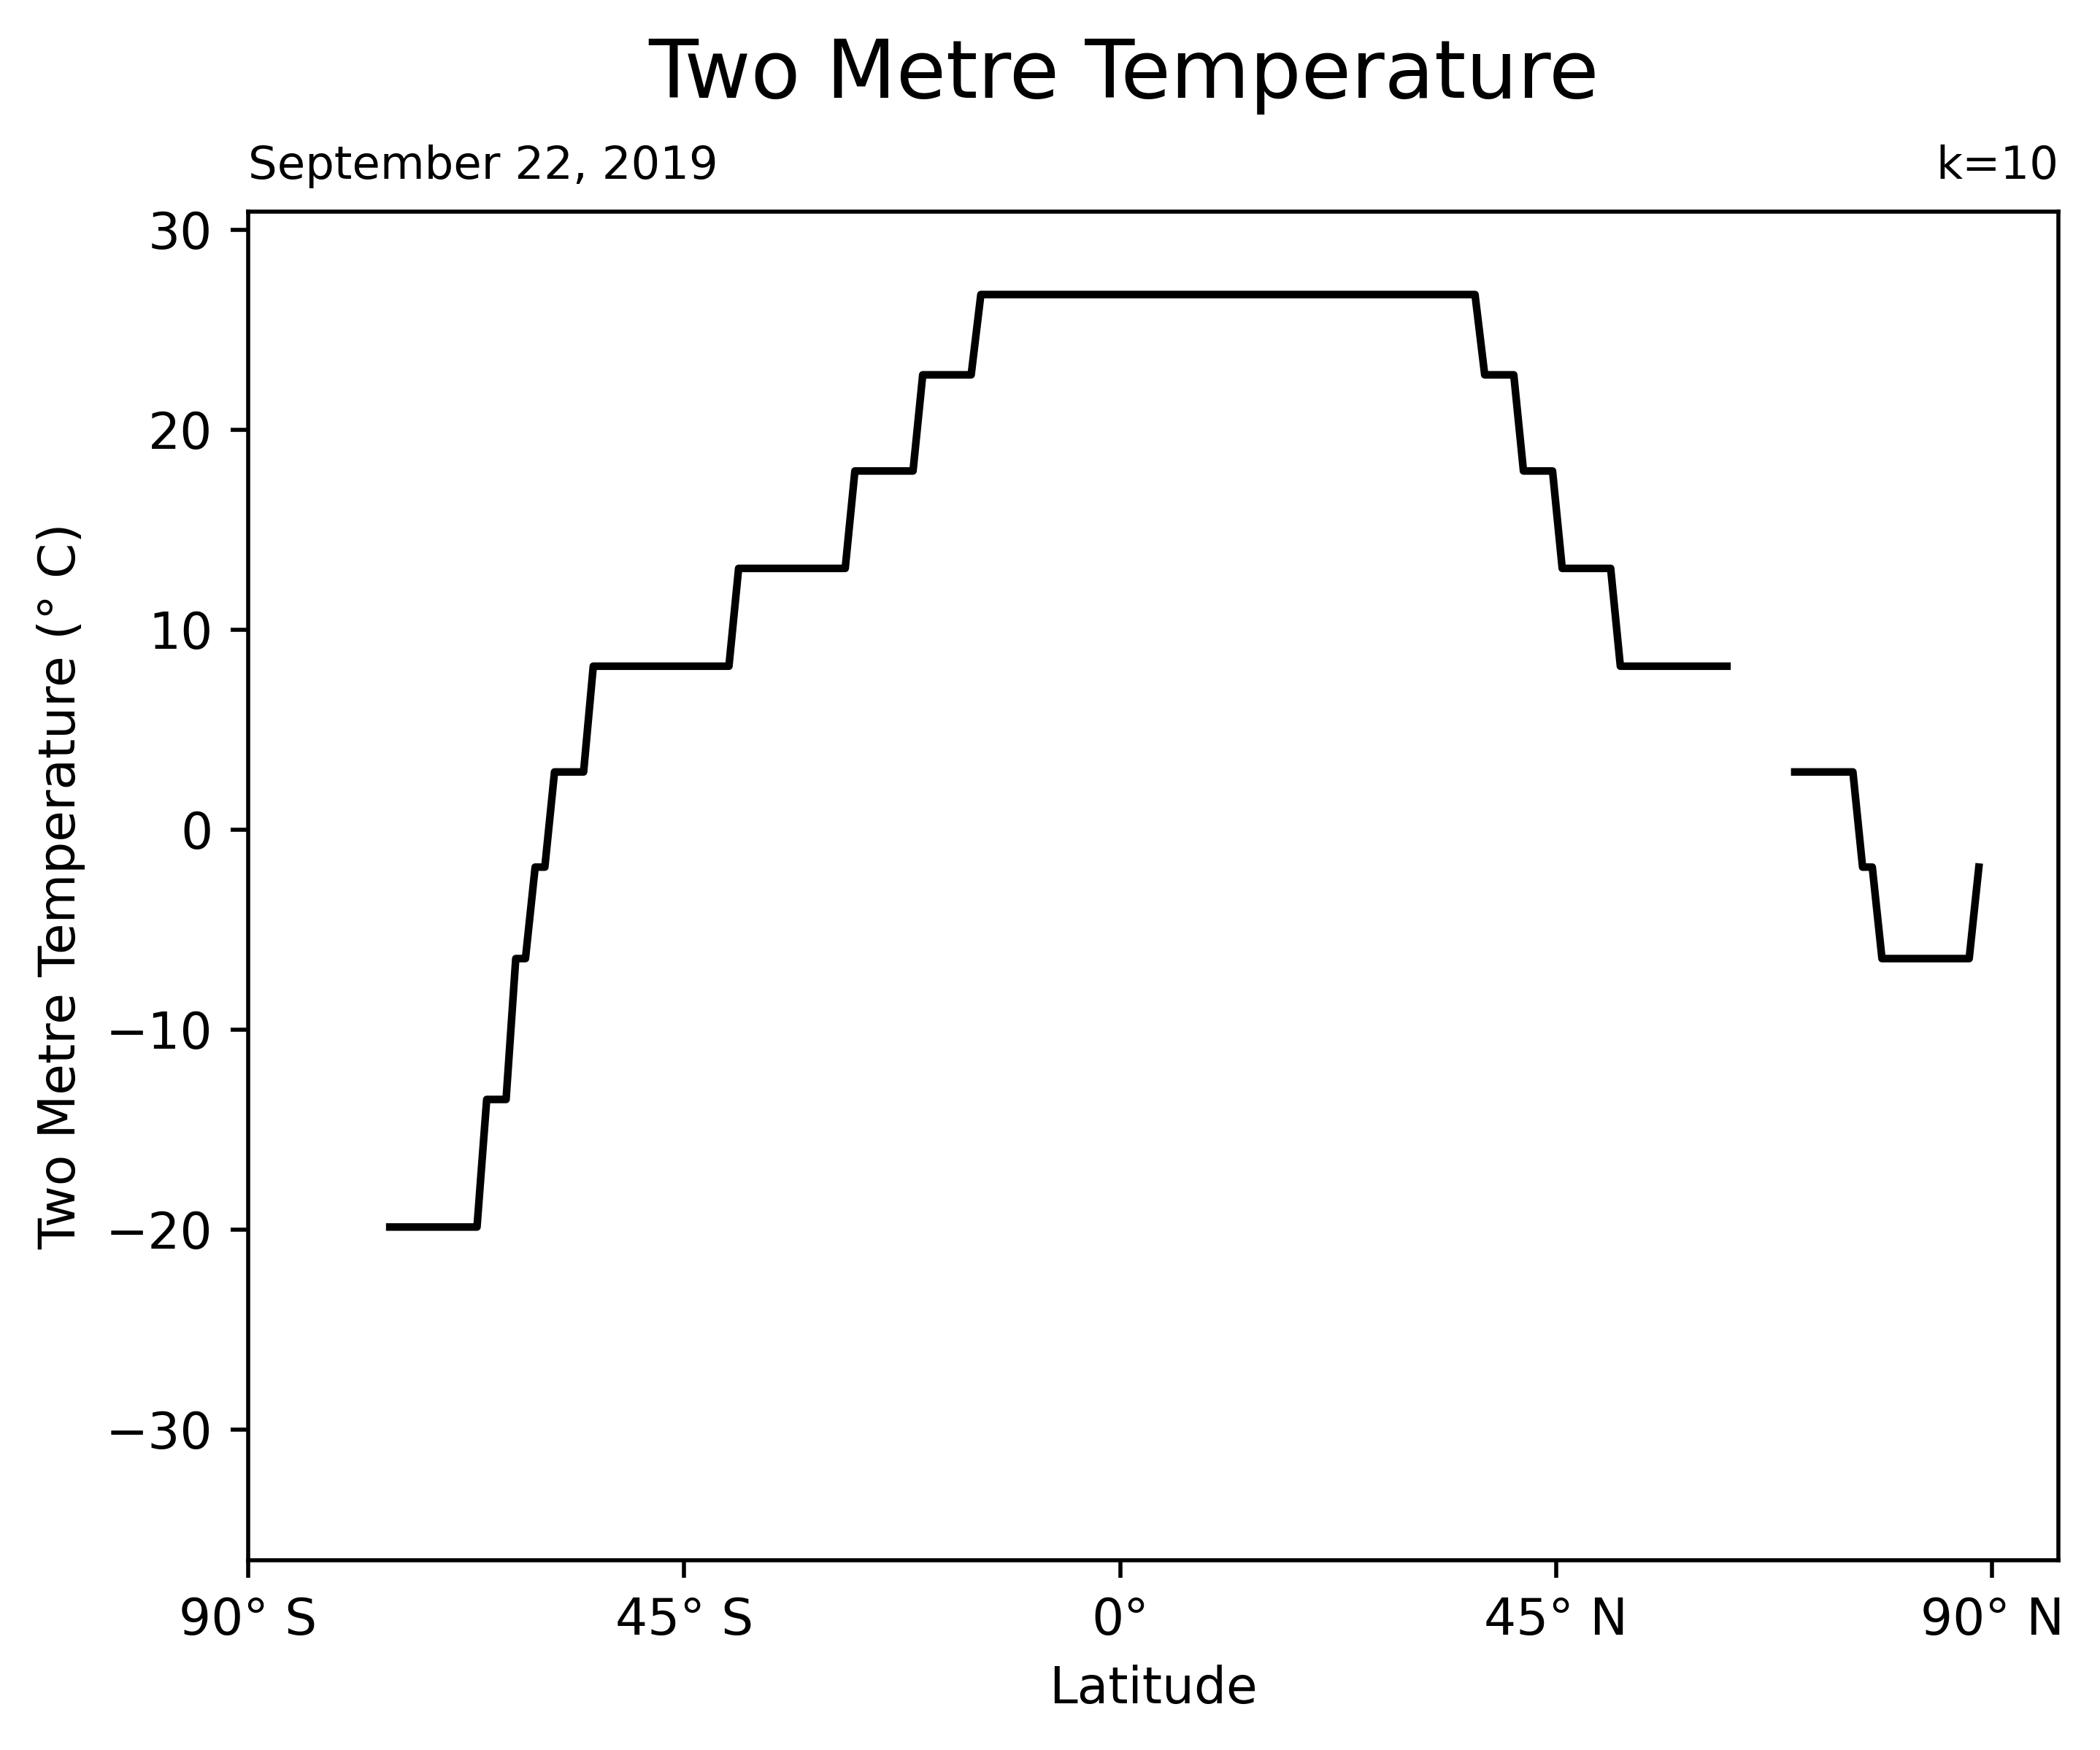
\includegraphics[width=0.5\textwidth]{figures/fig10.png}}
    \caption{Two Metre Atmosphere Temperature on September 22nd 2019.}
    \label{fig10}
\end{figure}


Using our line graph visualization we can see the clustering results in a completely different format. We observe similar trends as seen in the map plots. When comparing the sea surface temperature in Figure \ref{fig7} to Figure \ref{fig9} we see that on September 22nd in Figure \ref{fig9} the cluster with the coldest temperatures around 75º S is larger than the cluster with the coldest temperatures on March 20th in Figure \ref{fig7}. The opposite is the case for the cluster with the coldest temperatures around 85º N where Figure \ref{fig8} has more cold data points than the respective cluster in Figure \ref{fig9}. We also observe that the size of the cluster with the warmest temperatures increases significantly in both the sea surface temperature from Figure \ref{fig7} to Figure \ref{fig9} and two metre atmosphere temperature from Figure \ref{fig8} to Figure \ref{fig10}. Lastly, if we consider the overall position of the curve between Figure \ref{fig7} and Fib 7 and the curve between Figure \ref{fig8} and Figure \ref{fig10}, it is apparent that the entire curve is shifted farther south of the equator in Figure \ref{fig7} and Figure \ref{fig8} and farther north above the equator in Figure \ref{fig9} and Figure \ref{fig10}. When observing the two metre atmosphere temperature in Figure \ref{fig8} and Figure \ref{fig10} we notice significant differences in the temperatures at the south and north poles. In Figure \ref{fig8} we see that the coldest atmospheric temperature in the South Pole region is around -13º Celsius compared to the -20º Celsius in Figure \ref{fig10}. In Figure \ref{fig8} we see that the coldest atmospheric temperature in the North Pole is around -30º Celsius compared to the 0º Celsius in Figure \ref{fig10}.

Our observations on the difference in temperature at the polar regions at different times of the year, the sizes of the clusters, and the general shape of the line graphs can ultimately be explained by the movement of the sun. These shifts in atmospheric and sea surface temperature from lower latitudes to higher latitudes and vice versa are caused by the Sun. The Earth receives the highest amount of solar radiation at the point on the Earth's surface where the sun is directly overhead. This point moves north and south throughout the year, moving between the Tropics of Cancer at 23.4º N and the Tropics of Capricorn 23.5º S of the equator respectively \cite{b8}. The sun is directly overhead of the Tropics of Cancer during the vernal equinox on March 20th and directly overhead of the Tropics of Capricorn during the autumnal equinox on September 22nd. This explains the shift of sea surface and two metre atmosphere temperature between lower and higher latitudes throughout the year. When the sun is directly overhead the Tropics of Capricorn in the Southern Hemisphere on March 20th we see the largest shift of overall temperatures south of the equator. Similarly, when the sun is directly overhead of the Tropics of Cancer in the Northern Hemisphere on September 22nd we see the largest shift of overall temperatures north of the equator.

As observed from the changes in cluster locations in both sea surface temperature and two metre atmospheric temperature map plots, we notice that the location and sizes of the clusters shift more dramatically in the two metre atmosphere temperature plots than the sea surface temperature plots. This is due to the ocean being a large body of water that does a better job of absorbing and retaining temperature compared to less dense air. This causes the air temperature to increase and decrease at a faster rate from solar radiation when compared to the ocean water temperature.

% We have created two videos that show these changes dynamically. They can be found [cite to link].


\section{Conclusion}

In this paper, we proposed the f-clustering algorithm, an improved k-means clustering algorithm to cluster data in a single dimension. The proposed algorithm provided significant performance improvements over the well-known k-means algorithm as well as deterministic results. We then proved the correctness of our algorithm by showing it yields the same results as the traditional k-means algorithm. Using artificial datasets with randomly generated data we empirically analyzed the runtime of the algorithm, observing a runtime of $O(n \log n)$ in the worst case; an improvement over other improved k-means algorithms with a time complexity of $O(n^2)$ \cite{b1}. We then applied the proposed algorithm to a real-world dataset with oceanic and atmospheric data. To better understand the results of our algorithm and the data it produced we visualized the clusters on a map of the Earth as well as a discrete stepped line graph. We were able to observe trends in the size and locations of clusters on the Earth depending on the time of year.

A clear limitation of the proposed algorithm is that it can only be applied to data in a single dimension. Many datasets that benefit from clustering have a high-dimensionality. As such, a future improvement would be to extend the concepts used by the proposed algorithm to an algorithm that can be applied to high-dimensional data. A potential approach for this would be to generalize the concept of cluster borders to two or more dimensions using Voronoi diagrams, of which there exist efficient algorithms to compute and manipulate \cite{b10}.

Additionally, improvements can be made to the visualizations presented in this paper. First, the vertical line that appears at the prime meridian (0º longitude) could be removed. This gap in clusters was present even in early visualizations with unmodified data from the dataset. This could be fixed by determining why the data is not available, or interpolate data along the prime meridian to fill in the missing data. Second, the data point averaging algorithm that compresses the dataset could be improved to be more precise when considering masked values in the average calculations. This would result in clusters being plotted closer to land leaving a smaller gap between the edge of clusters and land.

There is a lot of future work related to the topics discussed in this paper that can be done. With the speed of the proposed algorithm combined with our visualization techniques, the visualizations could be expanded to be performed interactively in real-time. This would allow researchers to easily choose between the variable and number of clusters they want to visualize. Another area to expand on is the type of information that is visualized. The relationships between two or more dataset variables could be visualized by creating a function that takes multiple variables and computes a one-dimensional result to be visualized. This could help discover relationships between different components of the global environment such as the relationship between water temperature, air pressure, and air temperature. Another area for future work is parallelization. Because the proposed algorithm has the property that each cluster border will never cross each other it is possible to parallelize its execution by dividing the work into discrete chunks for separate processes to compute without any dependencies.

\begin{thebibliography}{00}
\bibitem{b1} K. A. Abdul Nazeer and M. P. Sebastian, "Improving the Accuracy and Efficiency of the k-means Clustering Algorithm" in Proceedings of the World Congress on Engineering, WCE 2009, London, U.K., July 1 - 3, 2009
\bibitem{b2} A. Likas et al., "The global k-means clustering algorithm", Pattern Recognition, vol. 36, no. 2, pp. 451-461, Feb. 2003
\bibitem{b3} A. M. Fahim et al., "An efficient enhanced k-means clustering algorithm", Journal of Zhejiang University-SCIENCE A, vol. 7, pp. 1626-1633, Oct. 2006
\bibitem{b4} C. Xie et al., "A survey on visual analysis of ocean data", Visual Informatics, vol. 3, no. 3, pp. 113-128, Sept. 2019
\bibitem{b5} S. Chattopadhyay, A. K. Das and K. Ghosh, "Finding patterns in the degree distribution of real-world complex networks: going beyond power law", Pattern Analysis and Applications, vol. 23, pp. 913-932, Apr. 2019
\bibitem{b6} I. Parberry, "The Pairwise Sorting Network", Parallel Processing Letters, vol. 02, no. 02n03, pp. 205-211, Mar. 1992
\bibitem{b7} D. Arthur et al., "Smoothed Analysis of the k-Means Method", Journal of the ACM, vol. 58, no. 5, pp. 1-31, Oct. 2011
\bibitem{b8} K. J. Feeley and J. T. Stroud, "Where on Earth are the "tropics"?", Frontiers of Biogeography, vol. 10, no. 1-2, Jul. 2018
\bibitem{b9} A. Kumar, Y. Sabharwal and S. Sen, "A simple linear time (1 + $\epsilon$)-approximation algorithm for k-means clustering in any dimensions," 45th Annual IEEE Symposium on Foundations of Computer Science, Rome, Italy, 2004, pp. 454-462, doi: 10.1109/FOCS.2004.7.
\bibitem{b10} S. Fortune, "A sweepline algorithm for Voronoi diagrams", Algorithmica, vol. 2, pp. 153-174, Nov. 1987
\end{thebibliography}

\end{document}
